% THIS IS AN EXAMPLE DOCUMENT FOR VLDB 2012
% based on ACM SIGPROC-SP.TEX VERSION 2.7
% Modified by  Gerald Weber <gerald@cs.auckland.ac.nz>
% Removed the requirement to include *bbl file in here. (AhmetSacan, Sep2012)
% Fixed the equation on page 3 to prevent line overflow. (AhmetSacan, Sep2012)

\documentclass[conference]{IEEEtran}
\usepackage{graphicx}
\usepackage{balance}  % for  \balance command ON LAST PAGE  (only there!)
\usepackage{subfigure}
\usepackage{caption}
\usepackage{url}
\begin{document}

% ****************** TITLE ****************************************

\title{YCSB-D: Benchmarking Adaptive Frameworks With Dynamic Workload Variations}

% possible, but not really needed or used for PVLDB:
%\subtitle{[Extended Abstract]
%\titlenote{A full version of this paper is available as\textit{Author's Guide to Preparing ACM SIG Proceedings Using \LaTeX$2_\epsilon$\ and BibTeX} at \texttt{www.acm.org/eaddress.htm}}}

% ****************** AUTHORS **************************************

% You need the command \numberofauthors to handle the 'placement
% and alignment' of the authors beneath the title.
%
% For aesthetic reasons, we recommend 'three authors at a time'
% i.e. three 'name/affiliation blocks' be placed beneath the title.
%
% NOTE: You are NOT restricted in how many 'rows' of
% "name/affiliations" may appear. We just ask that you restrict
% the number of 'columns' to three.
%
% Because of the available 'opening page real-estate'
% we ask you to refrain from putting more than six authors
% (two rows with three columns) beneath the article title.
% More than six makes the first-page appear very cluttered indeed.
%
% Use the \alignauthor commands to handle the names
% and affiliations for an 'aesthetic maximum' of six authors.
% Add names, affiliations, addresses for
% the seventh etc. author(s) as the argument for the
% \additionalauthors command.
% These 'additional authors' will be output/set for you
% without further effort on your part as the last section in
% the body of your article BEFORE References or any Appendices.

%\numberofauthors{3} %  in this sample file, there are a *total*
%% of EIGHT authors. SIX appear on the 'first-page' (for formatting
%% reasons) and the remaining two appear in the \additionalauthors section.
%
%\author{
%% You can go ahead and credit any number of authors here,
%% e.g. one 'row of three' or two rows (consisting of one row of three
%% and a second row of one, two or three).
%%
%% The command \alignauthor (no curly braces needed) should
%% precede each author name, affiliation/snail-mail address and
%% e-mail address. Additionally, tag each line of
%% affiliation/address with \affaddr, and tag the
%% e-mail address with \email.
%%
%% 1st. author
%\alignauthor
%Subhajit Sidhanta\\%\titlenote{Dr.~Trovato insisted his name be first.}\\
%       \affaddr{Louisiana State University}\\
%       %\affaddr{102F Electrical Engineering Building}\\
%       %\affaddr{Baton Rouge, LA, USA}\\
%       \email{ssidha1@lsu.edu}
%% 2nd. author
%\alignauthor
%Supratik Mukhopadhyay\\%\titlenote{Dr.~Trovato insisted his name be first.}\\
%       \affaddr{Louisiana State University}\\
%       %\affaddr{102F Electrical Engineering Building}\\
%       %\affaddr{Baton Rouge, LA, USA}\\
%       \email{supratik@csc.lsu.edu}
%% 3rd. author
%\alignauthor
%Wojciech Golab\\%\titlenote{Dr.~Trovato insisted his name be first.}\\
%       \affaddr{University of Waterloo}\\
%       %\affaddr{200 University Avenue West}\\
%       %\affaddr{Waterloo, Ontario, N2L 3G1, Canada}\\
%       \email{wgolab@uwaterloo.ca}
%}
% There's nothing stopping you putting the seventh, eighth, etc.
% author on the opening page (as the 'third row') but we ask,
% for aesthetic reasons that you place these 'additional authors'
% in the \additional authors block, viz.
%\additionalauthors{Additional authors: John Smith (The Th{\o}rv\"{a}ld Group, {\texttt{jsmith@affiliation.org}}), Julius P.~Kumquat
%(The \raggedright{Kumquat} Consortium, {\small \texttt{jpkumquat@consortium.net}}), and Ahmet Sacan (Drexel University, {\small \texttt{ahmetdevel@gmail.com}})}
%\date{30 July 1999}
% Just remember to make sure that the TOTAL number of authors
% is the number that will appear on the first page PLUS the
% number that will appear in the \additionalauthors section.

\author{\IEEEauthorblockN{Subhajit Sidhanta\IEEEauthorrefmark{1}, Supratik Mukhopadhyay\IEEEauthorrefmark{1}, and Wojciech Golab\IEEEauthorrefmark{2}}% and Saikat Basu\IEEEauthorrefmark{1}}
\IEEEauthorblockA{\IEEEauthorrefmark{1}Louisiana State University, Baton Rouge, Louisiana, USA, Email: \{ssidha1, supratik\}@csc.lsu.edu}
\IEEEauthorblockA{\IEEEauthorrefmark{2}University of Waterloo, Waterloo, Ontario, Canada, Email:  wgolab@uwaterloo.ca}}
\maketitle

\begin{abstract}
We demonstrate YCSB-D, a tool that builds upon YCSB (Yahoo Cloud Serving Benchmark suite) to assist users in simulating dynamic variations in  workloads. % through a web-based user interface. %The user interface comprises an input web form that allows users to specify dynamic variation patterns for a workload, and configure the workload parameters.
 YCSB-D allows users to run a sequence of YCSB workloads on a distributed datastore over long periods of time, without requiring users to manually change the workload configuration in  individual nodes each time the workload type needs to be modified.
  YCSB-D can be used to simulate  workloads in real world systems that use distributed datastores  (like Netflix, Youtube, Facebook, Amazon, BitTorrent, etc.), which reportedly exhibit different workload characteristics during different times of the day.  %We demonstrate that YCSB-D can simulate a typical  workload pattern for different use cases, characterized by different combinations of staleness and latency.
 Distributed datastores, operating under SLAs (Service Level Agreements), must adapt their configurations to such workload variations on a per-operation basis, to avoid SLA violations, in terms of the observed latency and staleness (i.e., how old the result is).  %YCSBD is integrated with OptCon, a framework that automatically tunes the target datastore on an per-operation basis, such that the observed latency and staleness satisfies the tolerance thresholds specified in the SLA.
 A considerable body of database and systems research aims at developing automated adaptive frameworks, that can tune distributed datastores to dynamic workload variations. %under performance thresholds specified in the SLAs.
  The dynamic workload variations simulated with YCSB-D can be used to evaluate the adaptability of such frameworks to changing workload characteristics. %, under a given SLA.
   We demonstrate the ability of YCSB-D to evaluate the adaptability of OptCon, an automated framework, that tunes the consistency settings of Cassandra with respect to the latency and staleness thresholds in an SLA.
\end{abstract}



\section{Introduction}

YCSB \cite{Cooper:2010:BCS:1807128.1807152} is widely used to simulate standard benchmark workloads for cloud-based systems, like Cassandra, MongoDB, Hbase, etc. \cite{Lakshman:2010:CDS:1773912.1773922,Chodorow:2010:MDG:1941134}. %These workloads are used to evaluate the performance of many distributed datastores that are typically used by cloud-based applications. The benchmark workloads are spawned as daemon processes from the target systems, like Cassandra, MongoDB, Hbase, etc.  \cite{Lakshman:2010:CDS:1773912.1773922,Chodorow:2010:MDG:1941134}, %, %,hbase2011george,
%%conf/sigmod/Sivasubramanian12}, %,Taylor:1998:JDR:521032},
%             running on top of representative cloud instances (like Amazon Ec2).
           % YCSB helps users collect various performance statistics for the operations performed by the target system.
           The YCSB suite comprises a workload generator, that can simulate a set of core workload types, characterized by parameters, like read-write proportions, request distribution, target throughput, etc., emulating different types of real world workload scenarios.
             To simulate scenarios where concurrent applications access the datastore from multiple nodes, YCSB can be set up to run as a collection of parallel client processes, where each node in a cluster runs a separate YCSB process. For executing YCSB in parallel mode, a user must manually start the YCSB workload executor from the command line at each individual node of the cluster. % target distributed datastore.
              Workloads in real world web-based applications (like Netflix, Youtube, Facebook, Amazon, BitTorrent, etc.), that use distributed datastores, widely vary over time \cite{NetflixWorkload-Variation}. Workload variation for such systems typically exhibit a specific pattern; the workload type varies in a characteristic fashion over time. For example, Netflix \cite{NetflixWorkload-Variation} observes that the network traffic for its applications reaches almost 37\% of Internet traffic during peak workload hours.
             For benchmarking such systems, a user must execute benchmark workloads for the
            target system in an uninterrupted back-to-back \emph{sequence}, following the characteristic workload variation pattern specific to the use case.
           \par We address the problem of allowing users to specify a back-to-back sequence of YCSB workloads, and execute the sequence in parallel in an uninterrupted manner. This involves the following sequence of steps to be performed at each individual node: 1) a given core workload is started from the YCSB command line, 2) after a specific time period the above workload must be stopped, 3) the next workload must be started, without any interruption (transition delay), from the command line, 3) iterate over step 1 to 2 uninterrupted, until the workload execution reaches the end of the benchmark period. The transition in step 2 must occur smoothly, without any interruption (delay), according to the characteristic variation pattern \cite{NetflixWorkload-Variation}. To execute a sequence of parallel workloads back-to-back, the YCSB process running in each individual node of a cluster needs to be stopped at the same time, and then simultaneously restarted at each node.
            \par  Performing the above sequence of steps at multiple nodes in a cluster at the same time, using the command line YCSB client can be difficult, even with YCSB++ \cite{Patil:2011:YBP:2038916.2038925}.
            For parallel YCSB processes executing on a cluster, YCSB++ uses ZooKeeper-based barrier synchronization to synchronize the client processes in individual nodes of the cluster.
            But YCSB++ does not support dynamically changing workloads. To run a different workload,
            the YCSB++ process at each node has to be manually stopped and restarted
            using the command line tool, which can result in transition delays.
             But the above transition from step 2 to step 3 must be instantaneous, to simulate smooth transition from one  workload to another.
               Hence, benchmark statistics generated using the above
              technique may not accurately reflect that in real world workload scenarios, which are typically characterized by smooth transition from one
               characteristic workload to another \cite{NetflixWorkload-Variation}. %The above steps need to be manually executed in each individual node of the target system.  In other words, part of the difficulty is starting and stopping processes at different hosts at the same time.
             %the user must follow the following steps: 1) manually start a workload type (as per the sequence) from the command line from each node, 2) wait for that workload type to finish execution, 3) then manually start the next workload type in the sequence, 4) iterate over steps 1 to 3 until the sequence is completed.
              %The state-of-the-art YCSB++ suite \cite{Patil:2011:YBP:2038916.2038925} allows only one core YCSB workload to be executed at a time.  To start a different core workload from the command prompt, the user must wait for the current workload to finish running, and manually start the new workload type. To execute each workload in the workload sequence uninterruptedly, the user must be able to anticipate (using sophisticated monitoring tools) exactly when each workload in the sequence finishes execution, and start the next workload immediately. There is no mechanism to bypass this manual process, and dynamically vary the workload types over a time period.
              We propose YCSB-D, a tool that allows users to automatically simulate a smooth variation pattern for parallel workloads executing
              over a target distributed datastore, running on a cluster of nodes. The tool allows users to
              specify a required pattern of variation in the workload over a given time period
              through an additional configuration parameter to the YCSB client. In addition, the tool can be used to
               simulate real world scenarios, where the workload transitions gradually over
               time according to a characteristic pattern.
               \par %However, for developing such a tool requires the  YCSB source code (particularly the YCSB client code in the core YCSB module) itself to be modified. %, which requires substantial understanding of the internal mechanism of YCSB.
               %the YCSB client
%               itself  has to be modified --- the control flow for executing YCSB workloads has to be altered; instead of executing a single workload for the whole time period over a given node, a client must execute a sequence of workloads.
                The control flow for YCSB is as follows: 1) the YCSB client module accepts workload configuration parameters, like number of
                threads, selected core workload, etc., from the command line, 2) the client module configures the selected core workload
                using the above parameters,  3) the client module instantiates the specified number of threads to execute
                the selected core workload, 4) the control is then passed to the workload executor which
                 executes the threads.
                %For allowing a sequence of different core
%                workloads to execute in the benchmark period, the above control flow in the source code has to
%                be altered.
                Since the selected core workload is configured and initialized by the client module before the
                control passes to the workload executor, only a fixed core workload can be executed at
                a time by YCSB.
                 YCSB-D integrates steps 2 and 3 with step 4, allowing the
                 YCSB executor module to configure, initialize, and execute a sequence of core workloads dynamically.
                 The above goal can not be achieved by: 1) tweaking the YCSB configuration files
                to specify the workload sequence, or by 2) developing a script, an interface layer, or a wrapper, to
                 execute the YCSB command line tool back-to-back with a different workload configuration each time. For
                 executing a sequence of YCSB workloads in parallel, the latter technique will require the users to
                 use the script/interface layer/wrapper to restart YCSB processes at each individual node in a cluster, that can result in
                 transition delays in the execution of the workload sequence.
                 %without actually touching the way the workloads are executed by the YCSB client.
               %  The YCSB source code (particularly the core YCSB module) needs to be modified, which requires substantial understanding of the internal mechanism of YCSB. %The above task is challenging, because of the size and complexity of the YCSB source code. %; the above modification can not be done in a short timespan by a developer who does not have deep insight of the YCSB source code.
            \par \textbf{Contribution:} We demonstrate  YCSB-D, a tool that can simulate \emph{dynamic} variations in YCSB workloads, and display the resulting variations in observed latency and throughput over time as a time series graph. YCSB-D provides a web-based user interface that comprises an input form that allows users to define a sequence of  YCSB workloads to be executed over a given time period. The user can divide the total duration of YCSB execution into a sequence of smaller time periods, and configure different YCSB workloads to be executed in each time period. The workload sequence is captured from the input form as a sequence of tuples; each tuple specifies a selected core YCSB workload type (a, b, c, etc.,) and its duration of execution. Users can  pass input parameters to YCSB-D, like number of threads, record count, request distribution, etc., along with a workload sequence.
            %The above sequence of workloads can be executed on top of a target system, and the variation in observed latency is displayed on a screen, along with other default YCSB outputs.
             YCSB-D only modifies the client module that configures the workloads to be executed, keeping the underlying
             architecture unchanged. Hence, YCSB-D  can work with any target system for which YCSB provides a connector
             (like Cassandra, Hbase, MongoDB, etc).
            \begin{figure}[!htbp]
        \centering
        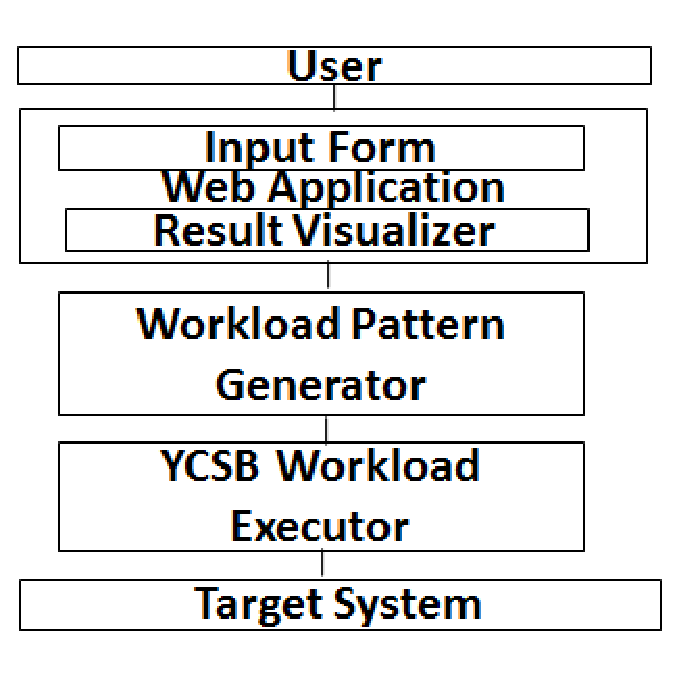
\includegraphics[width=1.6in,height=1.4in]
                    {arch.eps}
        \caption{The architecture of YCSB-D}
        \label{fig:Arch}
\end{figure}

%\begin{figure*}[!htpb]
%\centering
%%\noindent
%\subfigure[YCSB-D Client]{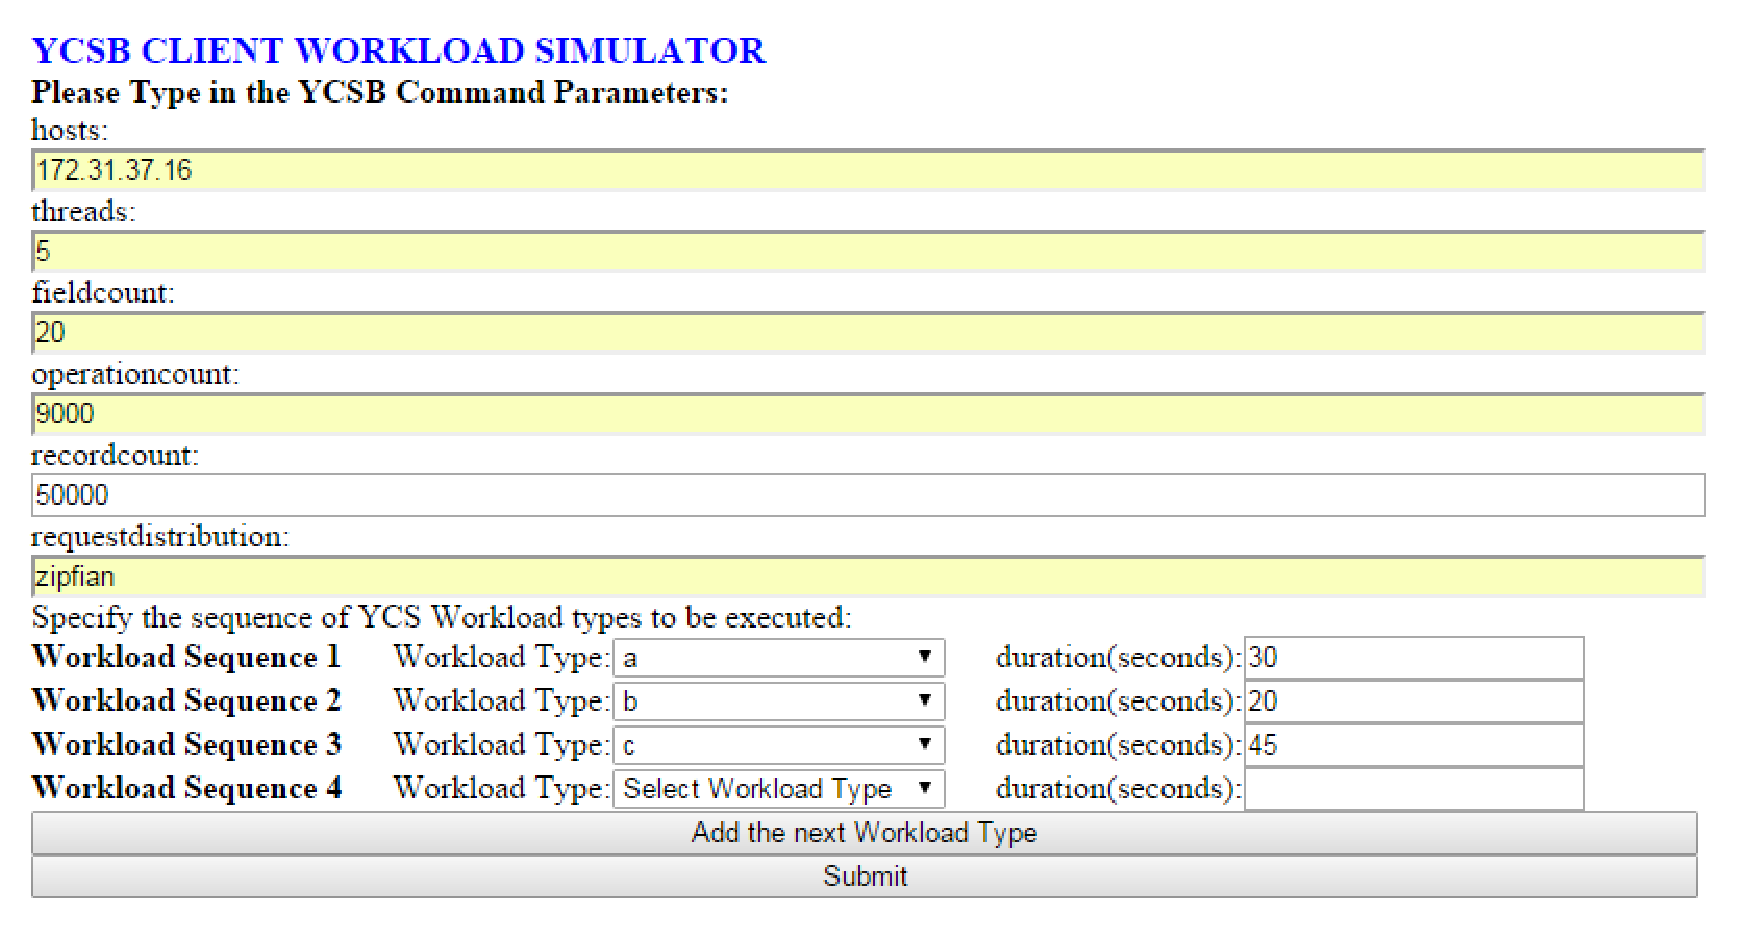
\includegraphics[width=0.48\linewidth,height=5cm]{ClientInput.eps}\label{fig:input}}\hfill
%\subfigure[YCSB-D Result Visualizer]{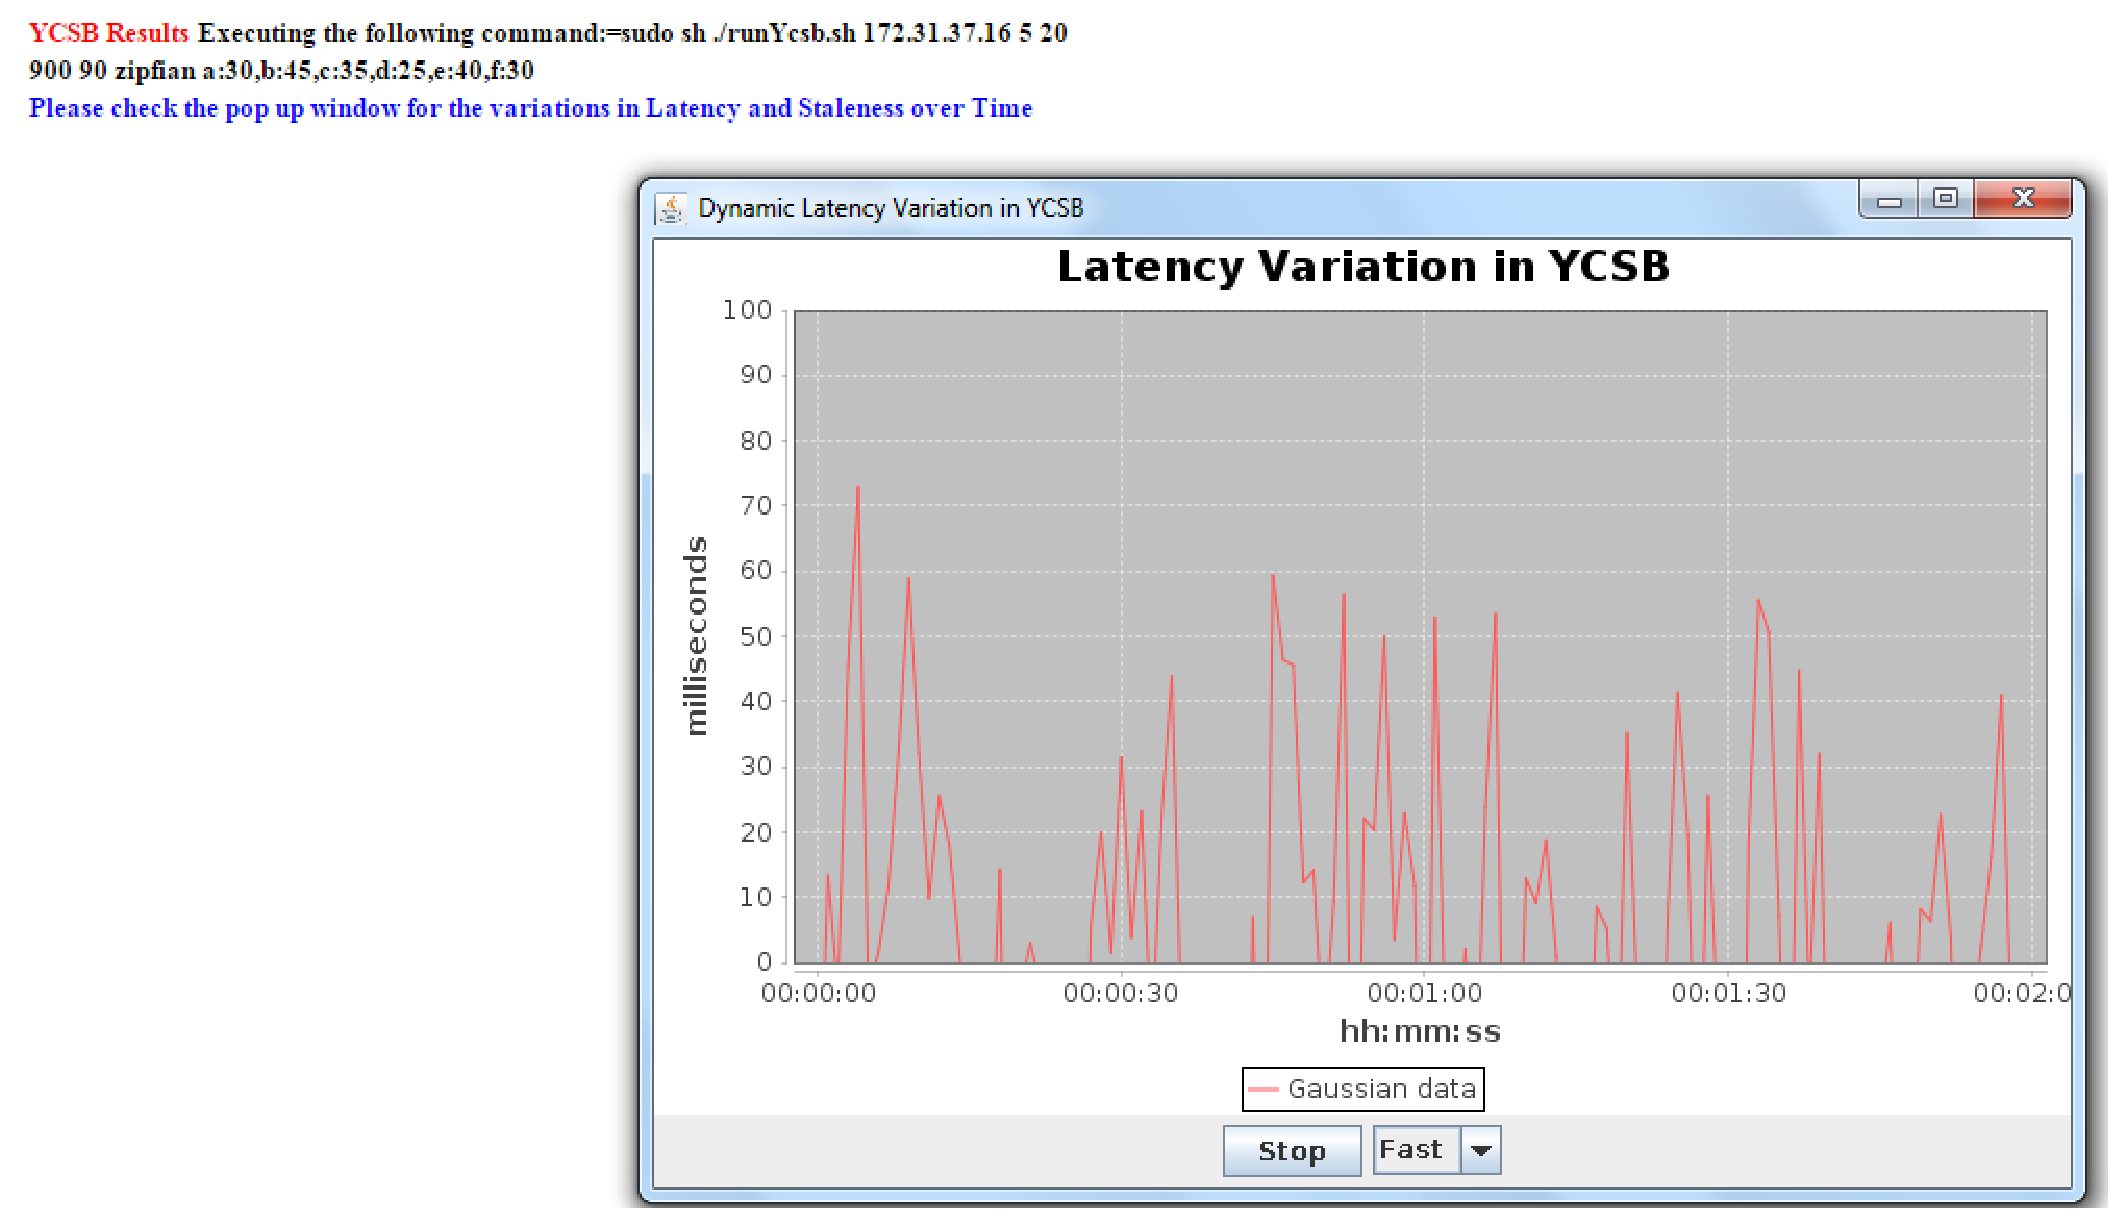
\includegraphics[width=0.48\linewidth,height=5cm]{Result.eps}\label{fig:outputut}}\hfill
%\caption{YCSB-D User Interface} \label{fig:impl}
%\end{figure*}

\begin{figure}[!htpb]%
       \centering%
        %\includegraphics[width=3.2in ,height=2.4in]{userstudy.eps}
        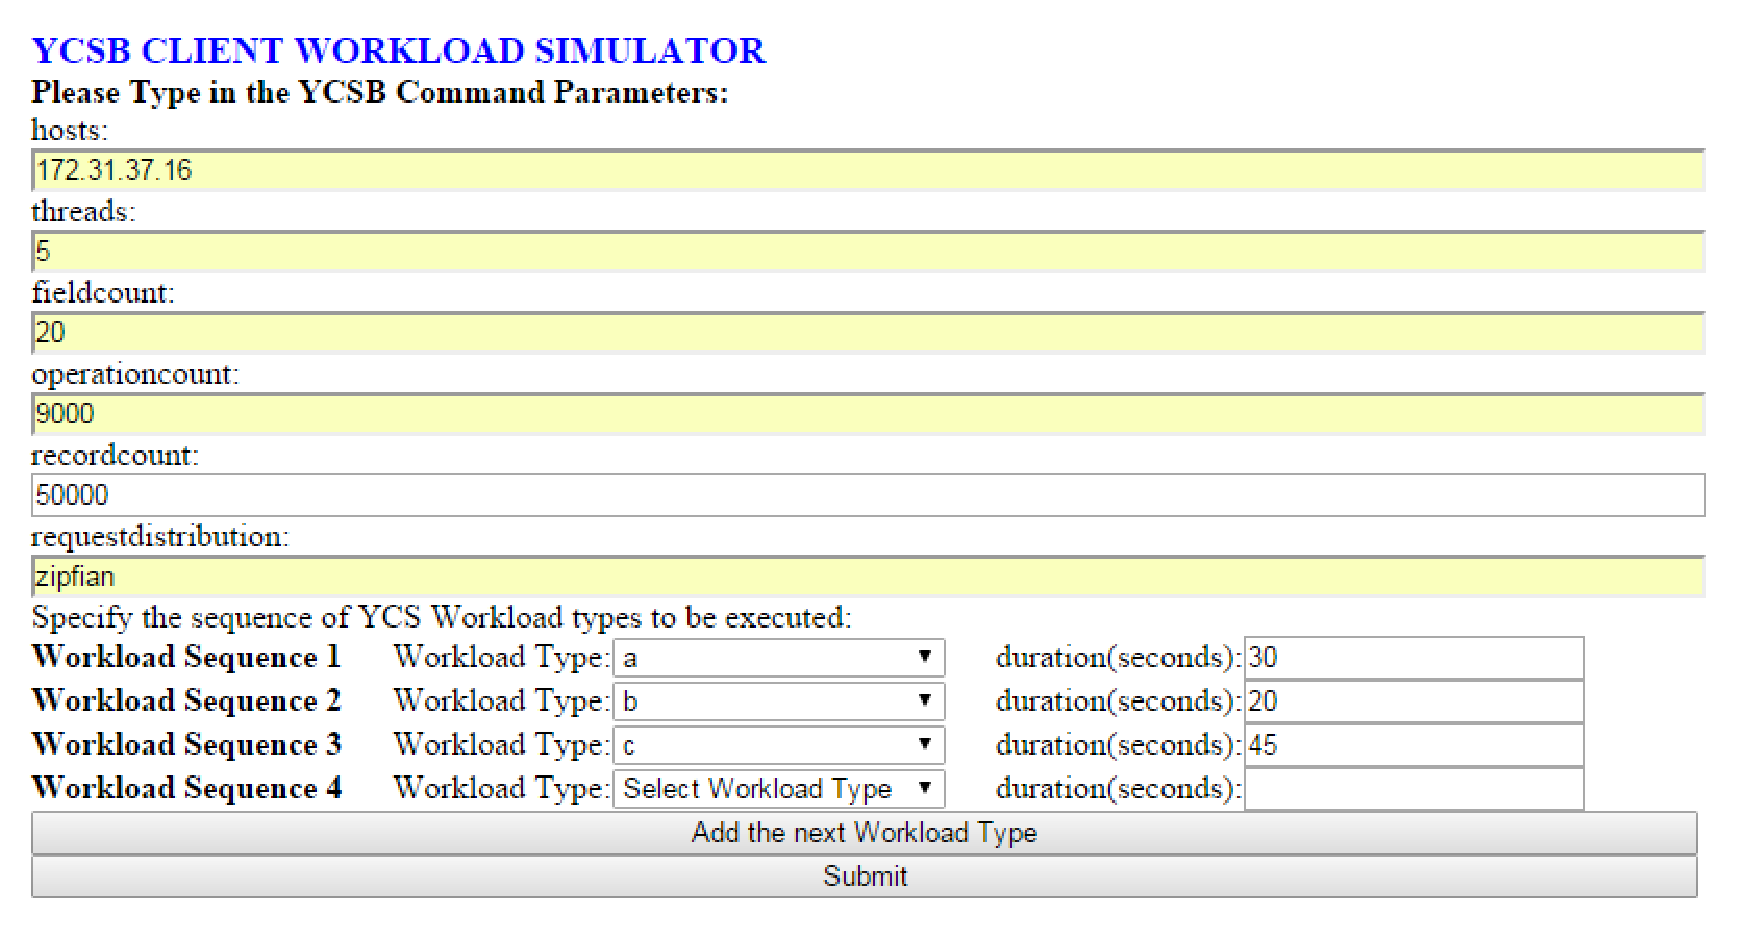
\includegraphics[width=8cm,height=5cm]
{ClientInput.eps}
        %\begin{gnuplot}[terminal=latex, terminaloptions=rotate]%        set xlabel "latency"
%        set ylabel "stalenes
%        set yrange [0:6]
%        plot 'sla1.csv' using 2:1 title 'fixed  consistency ANY WRITE/ONE READ' with points pt 1, 'sla1.csv' using 3:4 title 'predicted consistency' with points pt 3, 'sla1.csv' using 6:5 title 'fixed consistency READ/WRITE QUORUM' with points pt 2;
%        \end{gnuplot}
                \caption{YCSB-D User Interface}% under given subSLAs - a) s, b) SLA-2: latency 50ms, staleness 2.5ms, and c) SLA-3: latency 100ms, staleness 1ms}%
\label{fig:input}%
        \end{figure}%

         %   \par YCSB-D provides developers with the means to generate smooth workload variation patterns, echoing the workload variations in real world systems \cite{NetflixWorkload-Variation}, which use distributed datastores.  It allows developers to run an uninterrupted sequence of parallel YCSB workloads, % over long periods of time,
%             without requiring the users to manually stop and start the YCSB executor at each individual node (with changed workload configuration) each time a workload type needs to be modified. The ability to run many possible variation patterns in the YCSB workloads % for long periods of time
%             can assist developers in benchmarking the system behavior
             %in a more exhaustive fashion.% This, in turn, can help developers in producing better benchmarks.
             % Thus, YCSB-D can enable the developers to benchmark a system with realistic workloads, that vary over time.
             % YCSB-D can simulate different use cases, characterized by varying latency and throughput combinations, by dynamically varying the workload.
             \par %YCSBD allows developers to run an uninterrupted sequence of varying YCSB workloads over long periods of time, without manually stopping and starting the YCSB executor at each individual node (with changed workload configuration) each time a workload type needs to be modified. The ability to run YCSB workloads for long periods of time can assist developers in evaluating the adaptability of target systems to time-varying workload over long time periods.
              A considerable body of database and systems research \cite{conf/wecwis/YuV00, Terry:2013:CSL:2517349.2522731, Ardekani:2014:SGC:2685048.2685077} %, Sivaramakrishnan:2015:DPO:2813885.2737981}
                aims at developing automated adaptive frameworks, that can tune distributed datastores to adapt to workload variations, under performance thresholds specified in
              the SLAs. Such frameworks can automatically tune the consistency settings of an
              underlying datastore, thus helping the client applications satisfy the SLA under dynamic workload
              variations. Testing the adaptability of such frameworks requires benchmarking them with an exhaustive
              set of characteristic workload variations, simulated with YCSB, which is the standard benchmarking
              tool for distributed datastores. We propose leveraging the capability of YCSB-D to simulate possible
               variation patterns of YCSB workloads to evaluate the ability of an adaptive framework to adjust
               to dynamic workload variations, avoiding violation of the performance thresholds specified in the SLA.
               Thus, YCSB-D can effectively benchmark adaptive tuning frameworks \cite{conf/wecwis/YuV00, Terry:2013:CSL:2517349.2522731, Ardekani:2014:SGC:2685048.2685077} %, Sivaramakrishnan:2015:DPO:2813885.2737981}
                against varying workload characteristics, under a given SLA.
              Following \cite{Terry:2013:CSL:2517349.2522731}, we provide a metric \emph{$M$} to benchmark the adaptability of a target system to dynamic workload variations; $M$ is given as the percentage of the operations which did not result in SLA violations.
              %YCSB-D can simulate different use cases, characterized by varying latency and throughput combinations, resulting from varying the workload.
                For this demonstration, YCSB-D is integrated with OptCon \cite{OptCOnCCGRid2016}, an automated adaptive framework that can tune the consistency settings of a distributed datastore, such that the observed latency and staleness match the tolerance thresholds in the SLA, under a given workload and network condition.
                Among the adaptive tuning frameworks \cite{conf/wecwis/YuV00, Terry:2013:CSL:2517349.2522731, Ardekani:2014:SGC:2685048.2685077}, OptCon is the only open-source framework that we could find.
               We use the dynamic workload variations simulated with YCSB-D to benchmark OptCon's adaptability to varying workload, under the latency and staleness thresholds given in the SLA.
              % hence, we use OptCon to demonstrate YCSB-D.

\section{Design and Implementation}
 \textbf{Design:} Figure \ref{fig:Arch} presents the architecture of YCSB-D. YCSB-D modifies the code for the YCSB client, which involves complete restructuring of the execution flow of YCSB, allowing a sequence of workloads to be executed over  predefined time periods. YCSB-D comprises a client module that accepts input parameters from users, like number of threads, operation count, etc. The client module passes the input parameters to the Workload Generator module, which generates a sequence of YCSB workloads to be executed. The YCSB Workload Executor module executes the above workload sequence over a target system. The Result Visualizer module displays the variation in the observed latency and throughput over the duration of the execution of the workload sequence.
%\begin{table}[!htb]
%\centering
%\captionsetup{justification=centering}
%%\noindent
%\scalebox{0.8}{
%\begin{tabular}[b]{|c|c|} % centered columns (4 columns)
%\hline\hline %inserts double horizontal lines
% \bf Average Latency & \bf Staleness \\ % inserts table heading
% \hline\hline
% $\leq$100ms & $\leq$5ms \\ % inserting body of the table
% $\leq$50ms & $\leq$10ms \\
% $\leq$25ms & $\leq$15ms \\ % [1ex] adds vertical space
%\hline %inserts single line
%  %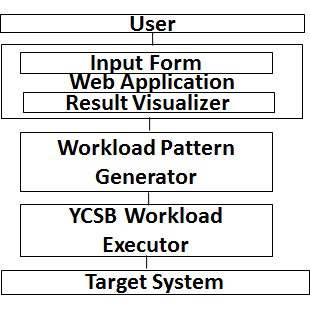
\includegraphics[width=1.5in,height=0.7in]{arch}
%\end{tabular}}
%\caption{Example subSLAs}\label{table:sla}
%\end{table}
%
% \par Like Terry et. al. \cite{Terry:2013:CSL:2517349.2522731}, users provide latency and staleness thresholds
% to OptCon in form of an SLA, illustrated in Table \ref{table:sla}. Each SLA consists of rows of \emph{subSLAs}, where each subSLA row, in turn, comprises two columns containing the thresholds for latency and staleness, respectively. Instead of
% categorical attributes %(such as eventual, read-my-writes, etc.)
%  \cite{Terry:2013:CSL:2517349.2522731}, OptCon uses threshold values for staleness \cite{DBLP:conf/cloud/GolabRAKWG13} in the subSLAs.
%% Terry et. al. uses SLAs structured as an ordered sequence of subSLA rows, ordered by the utility column. On the other hand, subSLAs
%% in OptCon are not necessary ordered.
% Unlike Terry et. al., subSLAs in OptCon do not have a utility column. Also, subSLAs are not necessary ordered. If the thresholds for a particular subSLA are violated, OptCon marks the operation as failed with respect to the given subSLA. Depending on the use case, the operation is retried against any of the next subSLA rows.  We  use the model $\mathcal{M}$ trained from Opcan predict a matching consistency level %workload, use case, and network state,
%   with respect to the given SLA thresholds for latency and staleness, under the current workload and network
%   state. A matching consistency is weak enough to satisfy the latency threshold, and simultaneously strong enough to satisfy the staleness threshold. We use the dynamic workload variations simulated with the YCSB tool to demonstrate OptCon's adaptability to workload variations.

\par \textbf{Implementation:}
 \def\tuple#1{\langle #1\rangle}
  YCSB-D implementation comprises two artifacts.
  1) A Java-based web application that comprises an input form that collects the input parameters from the users, and calls the YCSB-D client.
   2) A modified version of the YCSB framework that alters the source code of the YCSB client to accept a workload variation pattern.
       %\end{enumerate}
       3) A Workload Generator, that defines a sequence of core workloads to be executed over a given time period, and 4) a Workload Executor module that allows execution of a sequence of core workloads. %, instead of a fixed core workload.
        Figure \ref{fig:input} presents the web interface for YCSB-D. Figure \ref{fig:input} shows the input form, that the client module uses to submit the input parameters.
         Using the input form, the user can easily define workload variation patterns as follows. Users can choose a core workload type $w$ from a dropdown menu, and specify the duration of execution of $w$ in the adjacent text box. The dropdown menu allows users to select a workload from the choice of core workloads available in the YCSB suite. He can then add another workload type to the workload sequence, by clicking on the $\langle Add\; the\; Next\; Workload\rangle$ button, and specifying the workload type and duration as above. The workload sequence is captured by the web application as a sequence $c$ of tuples; each tuple $\tuple{w,d}$ comprises a character $w$ that represents the selected workload type, and a floating point parameter $d$ that denotes the duration for the execution of $w$. The above sequence $c$ is passed to the workload generator module, which then generates a sequence of core YCSB workloads to be executed.

%\section{Result Visualizer}

\par \textbf{Result Visualizer}
The Result Visualizer module comprises a web page that displays the observed latency and throughput for the benchmark operations in the form of a time series.
 From the viewpoint of the user of a distributed datastore, important performance parameters are  latency and client-observed \emph{consistency
anomalies} \cite{Terry:2013:CSL:2517349.2522731}, i.e., anomalies in the result of an operation observed by a client application.  Consistency anomalies are measured in terms of  client-centric \emph{staleness}
  \cite{Terry:2013:CSL:2517349.2522731}, %\cite{bayou},
   i.e., how stale (old) is the version of
 the data item (observed by a client application) with respect to the most recent version.
    The Result Visualizer also displays the observed consistency, i.e., staleness, computed in terms of the {\boldmath$\Gamma$} metric of Golab et. al. \cite{DBLP:conf/cloud/GolabRAKWG13}. As demonstrated in \cite{DBLP:conf/cloud/GolabRAKWG13}, {\boldmath$\Gamma$}  is preferred over other client-centric staleness measures for its proven sensitivity to workload parameters.
   %The metric $\Gamma$ %\cite{DBLP:conf/cloud/GolabRAKWG13}
    %is based upon Lamport's \emph{atomicity} property \cite{lamport_atomic}, which states that operations appear to
%	take effect in some total order that reflects their ``happens before'' relation in the following sense:
%	if operation A finishes before operation B starts then A must appear to take effect before B.
%We say that a trace of operations recorded by the logger is {\boldmath$\Gamma$}-atomic if it is atomic in Lamport's sense, or becomes atomic
%after each operation in the trace is transformed by decreasing its starting time by {\boldmath$\Gamma$}/2 time units, and increasing
%its finish time by {\boldmath$\Gamma$}/2 time units.
% In this context the start and finish times are shifted in a mathematical sense for the purpose of analyzing a trace, and do not imply injection of artificial delays;
%the behavior of the storage system is unaffected.
%%The $\Gamma$ metric can be defined at various granularity levels, including
%    \par The \emph{per-key $\Gamma$ score} quantifies the degree of client-centric staleness incurred by operations applied to a particular key. We use the $95^{th}$ percentile per-key $\Gamma$ score as the client-centric staleness measure. We order the per-key $\Gamma$ scores observed in a trace from lowest to highest and select the $(0.95*n)^{th}$ per-key $\Gamma$  value as the $95^{th}$ percentile per-key $\Gamma$, where $n$ is the total number of keys accessed in the trace. We considered average per-key  $\Gamma$, but settled for percentile per-key  $\Gamma$ since it takes into account the skewed nature of the workloads.
   %The variation in workload in typical web-based applications \cite{NetflixWorkload-Variation}, which use distributed datastores, is characterized by the observed latency and throughput at each instant in time.
%   Apart from staleness, the Result Visualizer  displays latency and throughput variation with change in YCSB workload. Most operations on distributed datastores are not instantaneous, but are executed over certain time intervals \cite{DBLP:conf/cloud/GolabRAKWG13}. Hence, following \cite{Bailis:2012:PBS:2212351.2212359}, we display the variations in the average latency over a time  interval of one minute.

\section{Demonstration}
 \textbf{Benchmarking Adaptive Tuning Frameworks}
 %Cloud-based applications and services, which use distributed datastores, often work under an SLA, that specifies certain performance thresholds
% that an application must satisfy.
  The performance of cloud-based applications and services, that use distributed datastores, is affected by the consistency
 settings applied to the datastore. According to the consistency setting applied, a distributed datastore waits for coordination
     among a specific number of replicas containing copies (i.e., versions) of the data item accessed by a given operation \cite{conf/sigmod/Sivasubramanian12}. %\cite{Lakshman:2010:CDS:1773912.1773922}.
      %If the
%     system waits for coordination among a smaller number of replicas the chance of getting a stale result (i.e., an older version) increases.
      With a weak consistency
  setting for an operation, the datastore waits for coordination among  a smaller number of replicas; hence there is a higher chance of yielding
   a stale result (since the most recent update may not have reached all the replicas through replica synchronization techniques).
   On the other hand, stronger consistency settings yield less stale results (more recent version), since they enforce coordination among a larger number of replicas.
    The latency for
      a given operation depends on the waiting time for the above coordination; hence, in turn, depends on the
       consistency setting applied. %For example, a
%   weak consistency setting for a read operation in Cassandra \cite{Lakshman:2010:CDS:1773912.1773922} requires only one of the replicas
%   to coordinate successfully, resulting in low latency and high chances of a stale read.
 Thus, both staleness
    and latency for an operation vary with the choice of consistency setting. The chosen consistency setting must be \emph{matching} with respect to the latency and staleness thresholds specified in the
 given SLA, i.e., it must be weak enough to satisfy the latency threshold, while being strong enough to satisfy the staleness threshold. A typical use case at Netflix \cite{NetflixWorkload-Variation} requires real-time response; hence the SLA
      typically comprises a low tolerance threshold for latency and a higher threshold for staleness. For the given SLA, under a peak-hour (prime-time) workload,
      the matching choice is a weak consistency setting. If the developer applies stronger consistency settings, the resulting high latency might violate the SLA.
 \par  To automate the process of consistency tuning in distributed datastores, a number of prototype
  adaptive tuning frameworks have been developed, like TACT \cite{conf/wecwis/YuV00}, Pileus \cite{Terry:2013:CSL:2517349.2522731}, Tuba \cite{Ardekani:2014:SGC:2685048.2685077}, %, Quela \cite{Sivaramakrishnan:2015:DPO:2813885.2737981},
   OptCon \cite{OptCOnCCGRid2016}, etc.
     Such frameworks can adapt the underlying datastore to variations in the workload, thus ensuring that the system always satisfies the SLA.
 However, testing such capabilities require the framework to be subjected to an exhaustive set of possible
 variations in the workload.
  We propose that the adaptability of such adaptive frameworks can be evaluated with dynamic variations in YCSB benchmark workload, simulated using the YCSB-D tool.
  YCSB-D can be used to simulate real world scenarios, characterized by specific patterns of workload variations.
  Thus, YCSB-D can be used to test if an adaptive framework can adjust the underlying datastore to satisfy the
  SLA under varying workloads; hence, YCSB-D can be used to benchmark the above mentioned adaptive frameworks.
  Following \cite{Terry:2013:CSL:2517349.2522731}, we quantify the adaptability of adaptive frameworks by the metric \emph{$M$}, which computes the percentage of operations which did not violate the SLA. %, and also stress test the target
%  system by simulating peak workloads under artificial network delays.
 \par \textbf{Demonstration  Setup:}
 OptCon \cite{OptCOnCCGRid2016} is an open-source example of an automated adaptive framework, that tunes Cassandra with respect to the latency and staleness thresholds in the SLA.
 We use YCSB-D to evaluate the adaptability of OptCon to dynamically varying YCSB workloads. The results obtained by running
 dynamically varying workloads (simulated with YCSB-D) on OptCon can be quantified in terms of the $M$-metric, that measures the adaptability of the framework (i.e., OptCon). YCSB-D is built as an extension of YCSB, which is a widely accepted
 benchmark for cloud-based systems and distributed datastores. Hence, YCSB-D can be used to evaluate adaptive
 frameworks that tune distributed datastores. However, OptCon is the only open-source available adaptive framework that we could find.   %OptCon is developed as a Java-based wrapper over Cassandra v2.1.0.  %\cite{Lakshman:2010:CDS:1773912.1773922}.
 %\\ \url{https://github.com/ssidhanta/YCSBpatchpredictconsistency/}, \\ \url{https://github.com/ssidhanta/TrainingModelGenerator/},
 The source code  for OptCon can be found at: \url{https://github.com/ssidhanta/HectorCient/}.
 %to demonstrate the ability of OptCon to adapt its the predicted  matching consistency levels to variations in workload.
%\subsection{Experimental Setup}\label{sec:setup}
 We have run  YCSB-D on a testbed of 20 Amazon ec2 small
instances, located in the same Ec2 region, running Ubuntu 13.10, loaded with Cassandra 2.1.2 %\footnote{Among the target systems  that are benchmarked with YCSB \cite{Cooper:2010:BCS:1807128.1807152}, Cassandra is the most widely used \cite{Lakshman:2010:CDS:1773912.1773922}. Hence, for demonstrating YCSB-D on OptCon, we use Cassandra as the representative datastore.} %Since YCSB-D modifies only the client module of YCSB, keeping the rest of the functionalities unchanged, it can work with any target system supported by YCSB.} %\cite{Lakshman:2010:CDS:1773912.1773922}
 with a replication factor of 3 (the number of replicas per data item).
  %However, YCSB-D is not specific to any target system, we use OptCon as an example for the demonstration. Technically, YCSBD can evaluate any automated system that can adapt to workload verification.
    %Our models are learnt from a training dataset comprising 23040 rows, and a testing dataset of 2560 rows, generated by running varying YCSB \cite{Cooper:2010:BCS:1807128.1807152} workloads.
%Cassandra nodes connected over a private intranet.
%We have developed the Logging module as an extension of the widely recognised YCSB \cite{Cooper:2010:BCS:1807128.1807152} benchmark tool
%(version 0.1.4) running on top of Cassandra 2.1.0.
 %The cluster consists of multiple disjoint nodes connected by a
%network with lags/time delays in the individual system clocks.
% Without time synchronization among the various nodes, the calculated measures like latency would be rendered
%useless because of the clock skew.
 %We have used the NTP (Network Time Protocol) protocol %\cite{Mills:1992:NTP:RFC1305}
% implementation from ntp.org to reduce the maximum clock skew to 5 ms; otherwise the clock skew in different nodes in the cluster may result in anomalies in the observed staleness.
  The demonstration can be accessed using the url: \url{http://ec2-52-36-221-215.us-west-2.compute.amazonaws.com:8080/YCSBDemo} %This
%accounts for a margin of 5 ms for error in the measurement. %, which is further reduced with averaging on multiple observations.
\begin{figure*}[!ht]
\centering
%\noindent
\subfigure[With OptCon; $M$ = $100$]{ 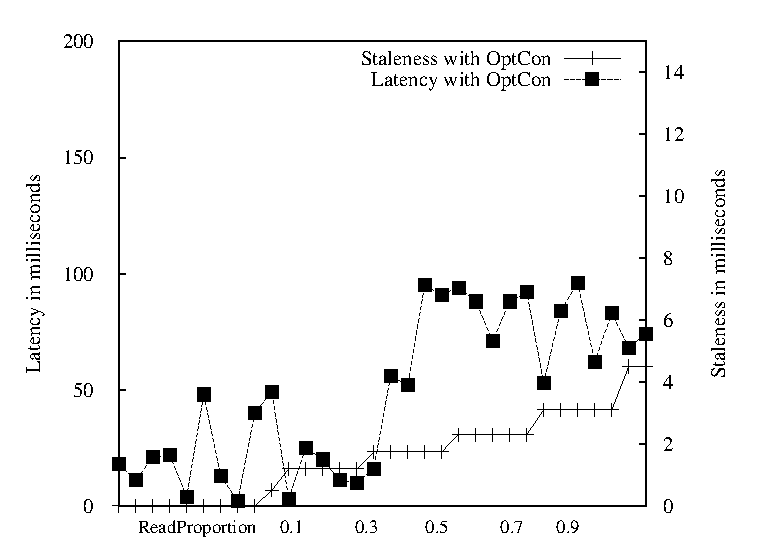
\includegraphics[width=0.3\linewidth,height=1.5in]{readVaryOptCon.eps}\label{loadVary}}\hfill
\subfigure[With Fixed Strong Consistency Settings; $M$ = $70$]{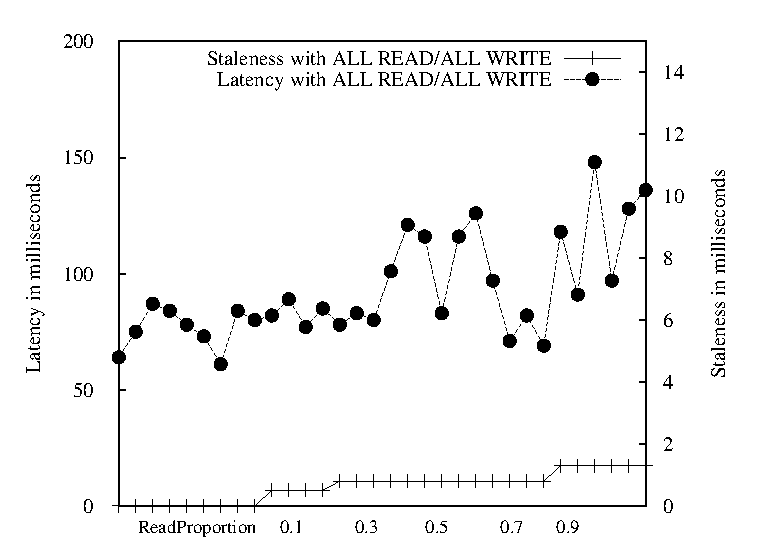
\includegraphics[width=0.3\linewidth,height=1.5in]{readVary1.eps}\label{strong}}\hfill
%\subfigure[Operations With READ ALL/WRITE QUORUM]{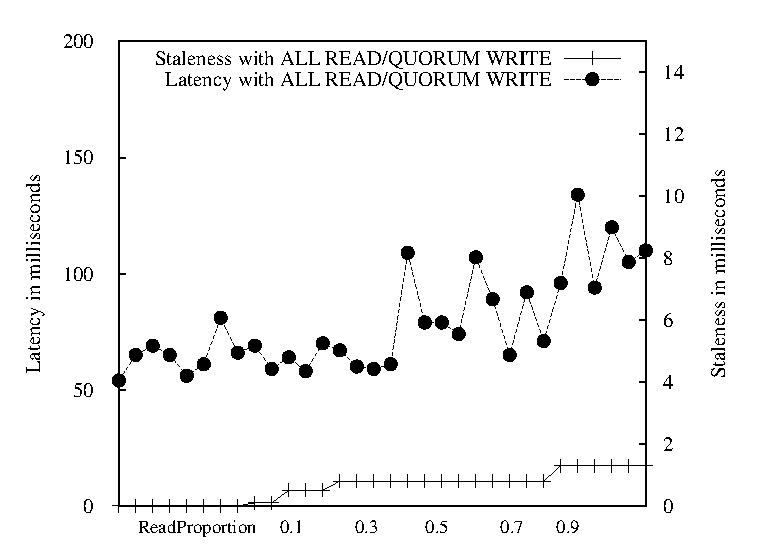
\includegraphics[width=0.3\linewidth,height=4cm]{readVary2.eps}\label{fig:label-5}}\hfill
%\subfigure[Operations With READ QUORUM/WRITE QUORUM]{ 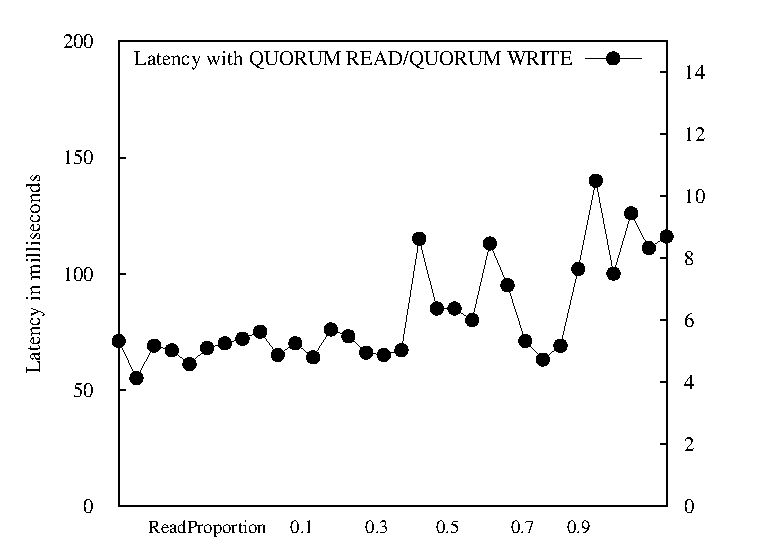
\includegraphics[width=0.3\linewidth,height=4cm]{readVary3.eps}\label{fig:label-6}}\hfill
%\subfigure[Operations With READ QUORUM/WRITE ALL]{ 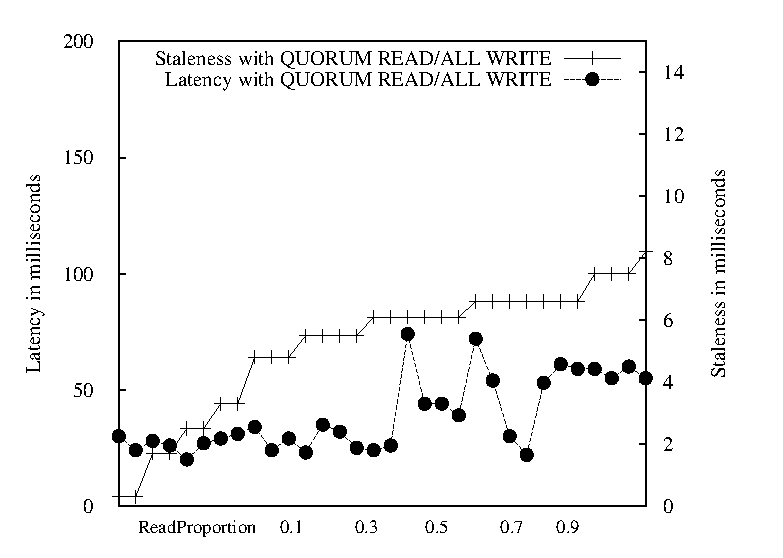
\includegraphics[width=0.3\linewidth,height=4cm]{readVary4.eps}\label{fig:label-7}}\hfill
%\subfigure[Operations With READ ALL/WRITE ANY]{ 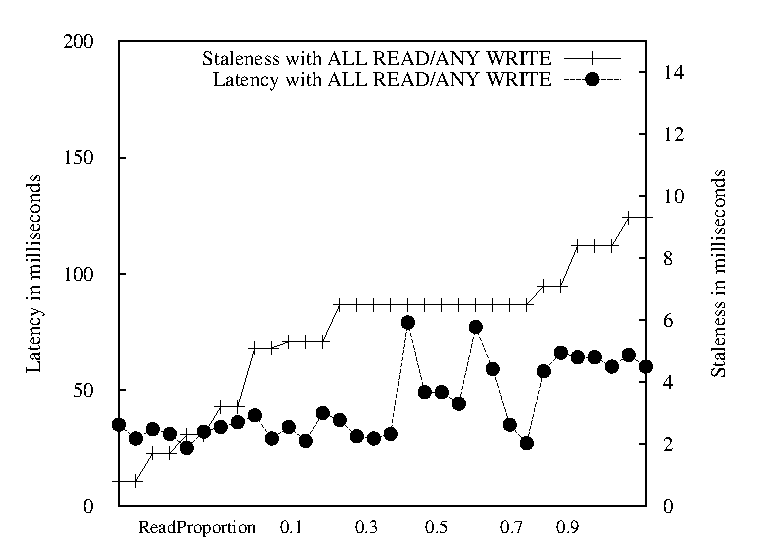
\includegraphics[width=0.3\linewidth,height=4cm]{readVary5.eps}\label{fig:label-8}}\hfill
%\subfigure[Operations With READ ALL/WRITE ONE]{ 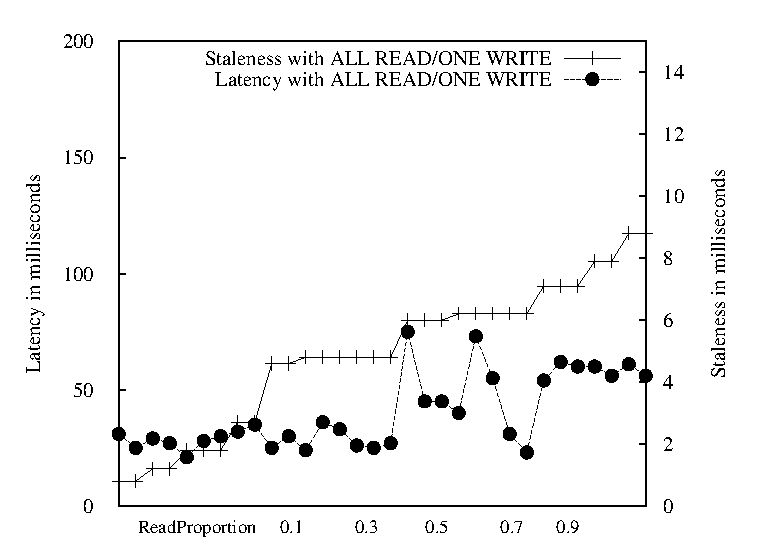
\includegraphics[width=0.3\linewidth,height=4cm]{readVary6.eps}\label{fig:label-9}}\hfill
%\subfigure[Operations With READ QUORUM/WRITE ANY]{ 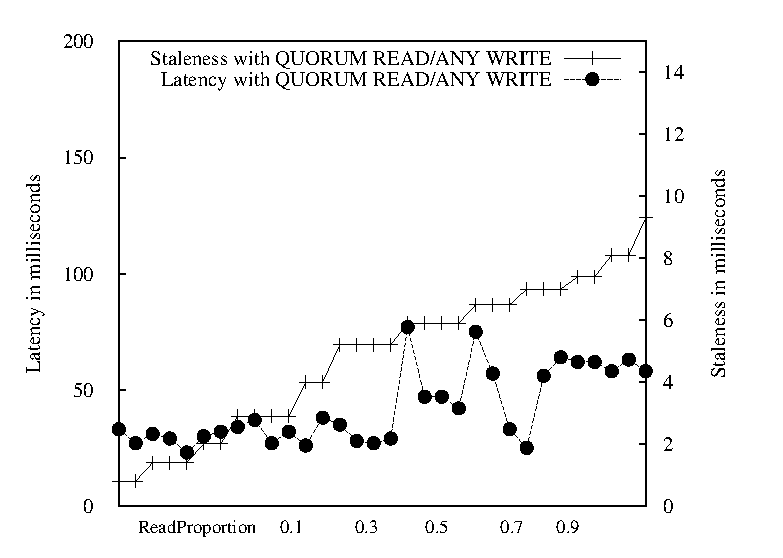
\includegraphics[width=0.3\linewidth,height=4cm]{readVary7.eps}\label{fig:label-10}}\hfill
%\subfigure[Operations With READ QUORUM/WRITE]{ 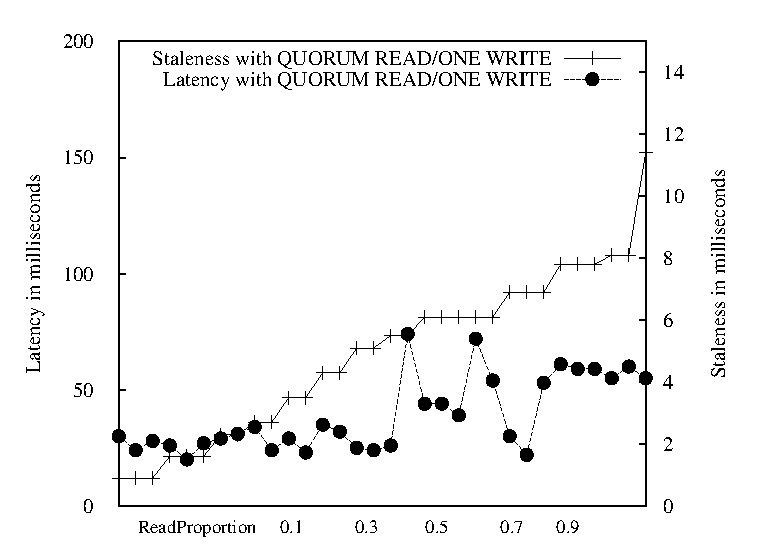
\includegraphics[width=0.3\linewidth,height=4cm]{readVary8.eps}\label{fig:label-11}}\hfill
\subfigure[With Fixed Weak Consistency Settings; $M$ = $45$]{ 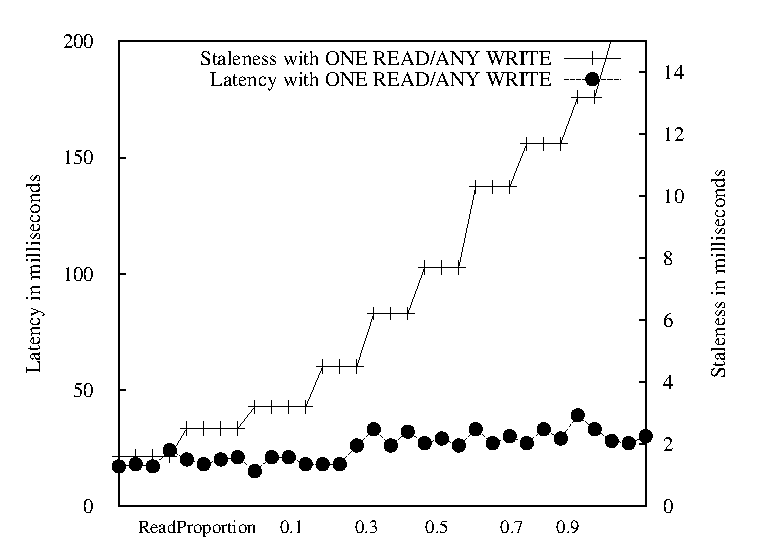
\includegraphics[width=0.3\linewidth,height=1.5in]{readVary9.eps}\label{weak}}\hfill
%\subfigure[Operations With READ ONE/WRITE QUORUM]{ 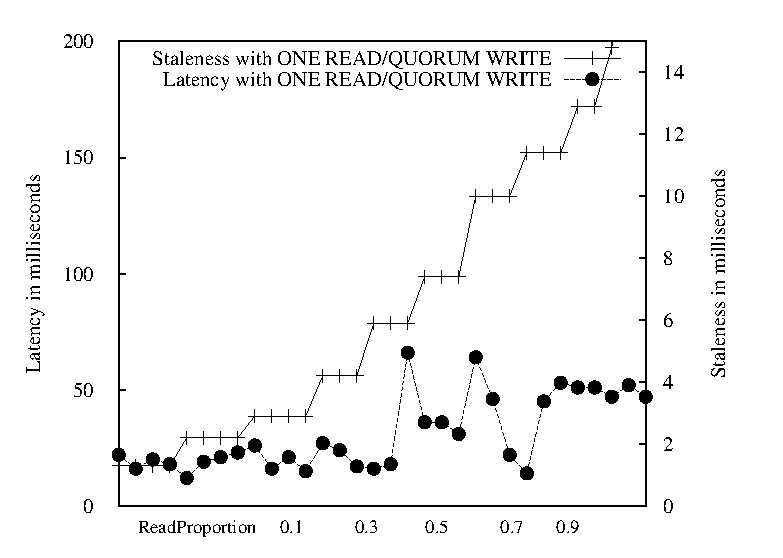
\includegraphics[width=0.3\linewidth,height=4.2cm]{readVary10.eps}\label{fig:label-13}}\hfill
%\subfigure[Operations With READ ONE/WRITE ALL]{ 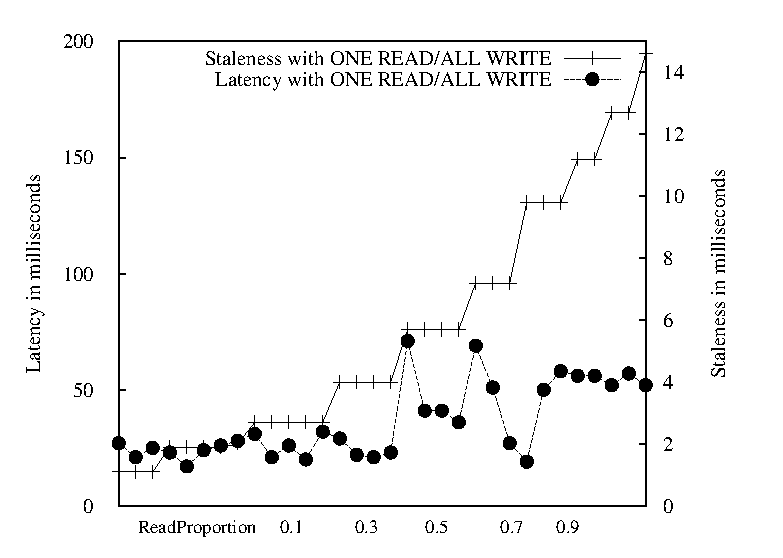
\includegraphics[width=0.3\linewidth,height=4.2cm]{readVary11.eps}\label{fig:label-14}}\hfill
\caption{Adaptability of OptCon to Varying Workload (Read Proportion) under the SLA (Latency:250ms Staleness: 5ms)}
%Manually chosen weak read-write consistency levels ONE/ANY are optimal (i.e., satisfy the subSLA) for low read proportions (i.e, in $<=55$\% cases) (Figures \ref{fig:label-8}, \ref{fig:label-9},
%\ref{fig:label-10}, \ref{fig:label-11}, \ref{fig:label-12}, \ref{fig:label-13}, and \ref{fig:label-14}). Manually chosen strong read-write consistency levels
%satisfy the subSLA for high read proportions (i.e, in $<=75$\% cases) (Figures \ref{fig:label-4}, \ref{fig:label-5}, \ref{fig:label-6}, and
%\ref{fig:label-7}).
%OptCon %is at least as effective as the optimal fixed consistency settings
% satisfies the subSLA (Figure \ref{fig:label-15}) for all possible read proportions by choosing the optimal consistency levels for each given read proportion.}
\end{figure*}
 %\begin{figure}[!htpb]%
%       \centering%
%        %\includegraphics[width=3.2in ,height=2.4in]{userstudy.eps}
%        \includegraphics[width=2.4in,height=1.8in]
%{loadVary.eps}
%        %\begin{gnuplot}[terminal=latex, terminaloptions=rotate]%        set xlabel "latency"
%%        set ylabel "stalenes
%%        set yrange [0:6]
%%        plot 'sla1.csv' using 2:1 title 'fixed  consistency ANY WRITE/ONE READ' with points pt 1, 'sla1.csv' using 3:4 title 'predicted consistency' with points pt 3, 'sla1.csv' using 6:5 title 'fixed consistency READ/WRITE QUORUM' with points pt 2;
%%        \end{gnuplot}
%                \caption{OptCon Adapts to Varying Workload: under the SLA thresholds: latency 20ms, staleness 5ms}%, b) SLA-2: latency 50ms, staleness 2.5ms, and c) SLA-3: latency 100ms, staleness 1ms}%
%\label{loadVary}%
%        \end{figure}%


\par \textbf{Demonstrating Adaptability of OptCon:}\label{sec:vary} %: Evaluation with Varying YCSB  ReadProportion}\label{sec:vary}
%We aim to make the case for varying YCSB workloads over time, to emulate different use cases.
 %Different use cases involve different acceptable thresholds for the observed latency. % and consistency, i.e., observed staleness.
%  Use cases like status updates, social voting, commenting, twitter, movie recommendation% (like the use case in \ref{fig:usecase})
%, etc. \cite{PlanetCassandra}, have a low tolerance threshold for latency. % and high tolerance threshold for staleness \cite{Terry:2013:CSL:2517349.2522731}. %,  eventual consistency might be appropriate as it would result in lower latency \cite{Terry:2013:CSL:2517349.2522731}.
% On the other hand, use cases, like customer order, bank accounting, log management systems, etc. \cite{PlanetCassandra}, work with mission critical data, that needs to be correct or complete at all times, can tolerate high latency. %Thus the consistency level needs to be tuned to satisfy the latency and staleness thresholds demanded by a particular use case.
% Similarly, for a real time operation  like web search \cite{PlanetCassandra}, a user may state that response time for any search query must not exceed 10 milliseconds \cite{Terry:2013:CSL:2517349.2522731}. %In this case, if the user applies a strong consistency level like ALL, a read operation will wait for all the replicas to respond, resulting in latency exceeding the given bound.
%  For banking applications \cite{PlanetCassandra}  that enable users to check account balance, withdraw or deposit funds, it is crucial that these actions do not leave the database in an incorrect state even for split second. In such cases, the application developer can accept higher values of latency.  %may want to put a low threshold of 5 milliseconds, on staleness of the values being read. %Weaker consistency settings like ANY will violate the given threshold.
% \par We demonstrate that YCSB-D can simulate all the above use cases, characterized by varying latency and staleness combinations, by dynamically varying the workload. %by tuning the
%read proportion (i.e., proportion of reads) parameter ($RW$) in the YCSB benchmark workloads
%(Figure \ref{fig:label-15}).
%We use Decision tree for the Learner module as it gives the best results with equal weight to accuracy and speed  (refer to Section \ref{sec:criteria}).
 %As per Table \ref{table:choice}, we choose the Decision tree  implementation of the Learner module.
  %We compare operations performed
%with OptCon, with those performed with manually chosen consistency levels.
  We demonstrate that YCSB-D can effectively evaluate the adaptability of OptCon to varying YCSB workloads. %, under latency and staleness thresholds specified in the SLA, using the metric $M$. %The user specifies the staleness and latency thresholds in the SLA to OptCon in a configuration file.
   YCSB workloads are executed on top of a Cassandra cluster, varying the core workload type using YCSB-D.
   The staleness and latency thresholds for a given SLA are supplied to OptCon in a configuration file.  In Figures \ref{loadVary}, \ref{strong},  and \ref{weak}
%through \ref{fig:label-12},
 we plot the read proportion for the workload along the x axis, the observed latency (obtained from the Result Visualizer) along the primary y axis, and the observed staleness (the {\boldmath$\Gamma$} values obtained from the Result Visualizer) along the secondary y axis.
 In Figure \ref{loadVary}, OptCon satisfies the SLA thresholds in $100\%$ cases; hence, $M$ = 100, whereas with manually chosen fixed consistency settings in Figures \ref{strong}  and \ref{weak}, $M$ is 70 and 45, respectively.
 This demonstrates that OptCon can adapt to varying workloads, tuning the consistency setting of the target datastore (Cassandra) according to the current workload.
  %We demonstrate that,
%Varying the read proportion ($RW$) in the workload from 0.1 to 1, we
% observe that a manually chosen read-write consistency level is optimal for only a fraction of the total number of cases.
 %under the subSLA SLA-1 (Table \ref{table:sla}).
% For a specific read proportion, only
% a subset of all possible read-write consistency levels is \emph{optimal}, i.e., satisfies latency and
% staleness thresholds in a given subSLA.
  %\par  According to the consistency setting applied, the distributed datastore waits for coordination
%     among a specific number of replicas containing copies (i.e., versions) of the data item accessed b the given operation \cite{Lakshman:2010:CDS:1773912.1773922}.
%      %If the
%%     system waits for coordination among a smaller number of replicas the chance of getting a stale result (i.e., an older version) increases.
%      With a weak consistency
%  setting for an operation, the datastore waits for coordination among smaller number of replicas \cite{Lakshman:2010:CDS:1773912.1773922}, hence has a greater chance of yielding
%   a stale result (since the most recent version may not have propagated yet to all the replica by replica synchronization \cite{Lakshman:2010:CDS:1773912.1773922}).
%   On the other hand, a stronger consistency level yields a less stale result (more recent version), since it enforces coordination among larger number of replicas \cite{Lakshman:2010:CDS:1773912.1773922}.
%    Also, the latency for
%      the given operation depends on the waiting time for the above coordination; hence, in turn, depends on the
%       consistency setting applied. %For example, a
%%   weak consistency setting for a read operation in Cassandra \cite{Lakshman:2010:CDS:1773912.1773922} requires only one of the replicas
%%   to coordinate successfully, resulting in low latency and high chances of a stale read.
% Thus, both the staleness
%    and latency for an operation vary with the choice of consistency setting. The chosen consistency setting must be \emph{matching} with respect to the latency and staleness thresholds specified in the
% given service level agreement (SLA), i.e., it must be weak enough to satisfy the latency threshold, while being strong enough to satisfy the staleness threshold. A typical use case of at Netflix \cite{NetflixWorkload-Variation} require real-time response \cite{NetflixWorkload-Variation}. Hence the SLA
%      typically comprises low latency and higher staleness thresholds. For the given SLA, workload, and
%      network state, the matching choice is a weak read-write consistency settings. If the developer applies stronger consistency settings, the resulting high latency would violate the SLA.
   \par  For a specific read proportion, only
 a subset of all possible consistency settings (ranging from strong to weak) is \emph{matching}, i.e., satisfies latency and
 staleness thresholds in a given SLA.  %OptCon can adapt to changing read proportion due to the presence of the parameter $RW$ as a feature in the prediction model $\mathcal{M}$. %Hence, a manually chosen fixed consistency level may not be matching for all possible read proportions.
 Under a given SLA, OptCon tunes the datastore with consistency settings chosen from the matching set of consistency settings for each read proportion (refer  Figure \ref{loadVary}).
  As shown by the results in \cite{DBLP:conf/cloud/GolabRAKWG13}, the frequency of stale results (i.e., higher
$\Gamma$ scores) increases with increasing read proportion in the workload.
Hence with higher read proportion, %, i.e.,
 $RW >$ 0.5 in
  in the right-half of the x axis (refer to Figure \ref{loadVary}), stronger read consistency settings are
  required to return less stale results. Hence fixed manually chosen strong consistency setting
   satisfies the SLA in the right-half of Figure \ref{strong}, whereas fixed weak consistency settings
   result in violation of the SLA in the right-half of Figure \ref{weak}.
%Also, since the proportion
% of writes is less, the penalty for the write latency overhead is less. Hence stronger write consistency settings, that result in high write latency, are acceptable.
  OptCon adapts to higher read proportion by tuning the datastore to operate under strong consistency settings, and satisfies the SLA for all read proportions of the workload in Figure \ref{loadVary}, i.e., $M$ = 100.  %Thus for higher read proportions, combinations of strong read-write consistency levels, i.e., ALL/QUORUM, succeed in lowering staleness values to acceptable bounds (right-half of the Figures \ref{fig:label-4}, \ref{fig:label-5}, \ref{fig:label-6},  and  \ref{fig:label-7}).  %Strong consistency levels achieve a maximum success rate of 75\% in satisfying the subSLA, with READ ALL/QUORUM WRITE (Figure \ref{fig:label-5}) and READ QUORUM/WRITE ALL (Figure \ref{fig:label-6}.
  %Taking into account the clock skew, the staleness is effectively 0 in these cases.  %But, weak read consistency settings result in high staleness values for  workloads with high read proportion.
   %For the same reasons, for higher read proportions, weak read consistency levels result in failure to achieve stringent staleness thresholds, as demonstrated by the points in the right-half of
%  Figures \ref{fig:label-8} through \ref{fig:label-14}. %Figures \ref{fig:label-4}, \ref{fig:label-5}, \ref{fig:label-6},   and
%  \ref{fig:label-7} demonstrate that the stronger manually chosen read-write consistency levels, i.e., ALL/QUORUM, succeed in lowering staleness values to acceptable bounds under high read proportion.
 With lower read proportions in the left-half of the x axes, the frequency of stale read results are smaller \cite{DBLP:conf/cloud/GolabRAKWG13}. In this case,
weaker consistency settings are sufficient for returning
consistent results. Hence, fixed weak consistency setting
   satisfies the SLA in the left-half of Figure \ref{weak}, whereas fixed strong consistency setting
   results in violation of the SLA in the left-half of Figure \ref{strong}. OptCon applies weak consistency settings to achieve the staleness and latency thresholds in the SLA for all workloads in Figure \ref{loadVary}.
  \par The latency and staleness plots in the Result Visualizer can be closely analyzed to observe whether OptCon can adjust to workload variations in a timely fashion, to eliminate the possibility of the users noticing SLA violations, in terms of the staleness and latency thresholds.
 Thus, YCSB-D  can be used to obtain deeper insights on the adaptability of automated tuning frameworks against real time variations in workload.
  The database and systems community can benefit from YCSB-D, which can serve as a benchmarking tool for
  testing the ability of a framework to adapt a target datastore to variations in
  workload. %, with respect to the benchmark metric $M$.
   %Figures \ref{fig:label-4}
%through \ref{fig:label-12} demonstrate that YCSB-D can be used to generate different YCSB workloads, characterized by different read proportions.
%Under different YCSB workloads, YCSB-D produces different combinations of latency (refer to the latency variations in Figures \ref{fig:label-4}
%through \ref{fig:label-12}), with different consistency levels applied.
% The different latency values characterize different real world workload scenarios, each of which are identified by a typical  workload variation pattern. Thus, YCSB-D can effectively simulate various workload scenarios, echoing the typical workload variation patterns of real world target systems. %In this case,
%weaker manually chosen read-write consistency levels, i.e., ONE/ANY (left-half of Figures \ref{fig:label-8} through \ref{fig:label-14}) are sufficient for returning
%consistent results. For lower read proportions, stronger consistency levels, i.e., ALL or QUORUM, are unnecessary,
%only resulting in high latency overhead.
%With weak consistency levels, we observe a maximum success rate of only $<=55$\% in  satisfying the subSLA (left-half of Figure \ref{fig:label-12})).
%Thus under lower read proportions, weaker manually chosen consistency levels, i.e., ONE/ANY, give better results, i.e., both lower staleness and lower latency, than ALL or QUORUM settings.
%     A particular manually chosen fixed consistency setting can satisfy staleness and latency thresholds in a given SLA for only certain workloads.
%% Strong consistency levels are suitable for higher read proportions, while weaker consistency is sufficient for lower read proportions.
%  Thus, manually chosen consistency levels show a maximum success rate of 75\% in satisfying the subSLA, with READ ALL/QUORUM WRITE (Figure \ref{fig:label-5}). %and READ QUORUM/WRITE ALL (Figure \ref{fig:label-6}.
% in contrast with a $100$\% success rate demonstrated by OptCon (Figure \ref{fig:label-15}).
%Thus, OptCon is more effective than any manually chosen consistency level in adapting to workload variations.

%\subsection{YCSB Core Workload Variations}
    %\begin{figure}[!htpb]%
%       \centering%
%        %\includegraphics[width=3.2in ,height=2.4in]{userstudy.eps}
%        \includegraphics[width=2.6in,height=2in]
%{loadVary}
%        %\begin{gnuplot}[terminal=latex, terminaloptions=rotate]%        set xlabel "latency"
%%        set ylabel "stalenes
%%        set yrange [0:6]
%%        plot 'sla1.csv' using 2:1 title 'fixed  consistency ANY WRITE/ONE READ' with points pt 1, 'sla1.csv' using 3:4 title 'predicted consistency' with points pt 3, 'sla1.csv' using 6:5 title 'fixed consistency READ/WRITE QUORUM' with points pt 2;
%%        \end{gnuplot}
%                \caption{Performance With Variation of Core Workload Type}% under given subSLAs - a) SLA-1: latency 20ms, staleness 5ms, b) SLA-2: latency 50ms, staleness 2.5ms, and c) SLA-3: latency 100ms, staleness 1ms}%
%\label{loadVary}%
%        \end{figure}%
%%First we demonstrate the performance of OptCon with respect to variations in workload.
% \par In Figure \ref{loadVary}, we
% make sequential runs of various YCSB workloads - the core workloads, namely a, b, c, d, e, f, and
% Hot Spot Workloads (multiple
% transactional load) over a Cassandra cluster of seven large Amazon m3 instances, with replication factor of 3.
% %We present a
%% scatter plot (refer ) displaying the latency and staleness/observed consistency
%% (represented by the average {\boldmath$\Gamma$} score, i.e., the average of the per key
%%        {\boldmath$\Gamma$}).
%  Figure \ref{loadVary} demonstrates that YCSB-D can simulate dynamic variation patterns comprising all possible core YCSB workloads. The different core YCSB workloads represent different real world workloads for distributed datastores. Thus, YCSB-D can be used to simulate the workload of any distributed datastores, that can be characterized by the different  YCSB core workload types.
 %We use different three subSLA rows:
% \begin{enumerate}
%  \item SLA-1 with 20 ms threshold for latency and 5 ms for staleness,
%  \item SLA-2 with 50 ms threshold for latency and 2.5 ms for staleness, and
%  \item SLA-3 with 100 ms threshold for latency and 1 ms for staleness.
%  \end{enumerate}
   %It can be
%  observed from the plot that OptCon outperforms fixed
%   consistency settings in terms of satisfying the various subSLA thresholds. For example,
%   \begin{itemize}
%  \item  under the fixed
%  consistency level ONE READ/ANY WRITE the three subSLA's fail under all YCSB workloads,
%  \item with READ/WRITE
%   QUORUM, SLA-1 breaks under all possible workloads,
%   \item SLA-2 breaks under YCSB workload f and Hot Spot workloads,
%   \item with ALL READ/QUORUM WRITE, SLA-1 and SLA-2 fails for all possible workloads, and
%   \item SLA-3 fail under YCSB workloads d and e.
%   \end{itemize}
    %On the other hand, OptCon
%    \begin{itemize}
%   \item satisfies the subSLA SLA-1 for all workload types, only breaking
%   down under Hot Spot workloads, on the ground that the staleness exceeds the 5 ms threshold,
%    \item succeeds in satisfying SLA-2 for all YCSB workloads except for Hot Spots (latency at Hot Spot exceeds the 50 ms threshold).
%   \item satisfies the subSLA SLA-3 works for workload types a, b, c, e, f, and Hot Spot, but fails under workload d.
%   \end{itemize}
 %  This shows that a particular subSLA may not be suitable for all possible workloads - the framework
%   must work with a specific subSLA particularly designed according to the use case (defined here by the
%   workload nature).
    %This makes the case for varying the benchmark workload over time, to emulate the different use cases represented by the different subSLAs. % for different
%    use cases, and a prediction framework (like ours) that can act upon the given subSLA and predict the matching consistency
%    level for the workload type.


%The \textit{proceedings} are the records of a conference.
%ACM, as well as PVLDB, seeks to give these conference by-products a uniform,
%high-quality appearance.  To do this, ACM / PVLDB has some rigid
%requirements for the format of the proceedings documents: there
%is a specified format (balanced  double columns), a specified
%set of fonts (Arial or Helvetica and Times Roman) in
%certain specified sizes (for instance, 9 point for body copy),
%a specified live area (18 $\times$ 23.5 cm [7" $\times$ 9.25"]) centered on
%the page, specified size of margins (2.54cm [1"] top and
%bottom and 1.9cm [.75"] left and right; specified column width
%(8.45cm [3.33"]) and gutter size (.083cm [.33"]).
%
%The good news is, with only a handful of manual
%settings\footnote{Two of these, the {\texttt{\char'134 numberofauthors}}
%and {\texttt{\char'134 alignauthor}} commands, you have
%already used; another, {\texttt{\char'134 balancecolumns}}, will
%be used in your very last run of \LaTeX\ to ensure
%balanced column heights on the last page.}, the \LaTeX\ document
%class file handles all of this for you.
%
%The remainder of this document is concerned with showing, in
%the context of an ``actual'' document, the \LaTeX\ commands
%specifically available for denoting the structure of a
%proceedings paper, rather than with giving rigorous descriptions
%or explanations of such commands.
%
%\section{The {\secit Body} of The Paper}
%Typically, the body of a paper is organized
%into a hierarchical structure, with numbered or unnumbered
%headings for sections, subsections, sub-subsections, and even
%smaller sections.  The command \texttt{{\char'134}section} that
%precedes this paragraph is part of such a
%hierarchy.\footnote{This is the second footnote.  It
%starts a series of three footnotes that add nothing
%informational, but just give an idea of how footnotes work
%and look. It is a wordy one, just so you see
%how a longish one plays out.} \LaTeX\ handles the numbering
%and placement of these headings for you, when you use
%the appropriate heading commands around the titles
%of the headings.  If you want a sub-subsection or
%smaller part to be unnumbered in your output, simply append an
%asterisk to the command name.  Examples of both
%numbered and unnumbered headings will appear throughout the
%balance of this sample document.
%
%Because the entire article is contained in
%the \textbf{document} environment, you can indicate the
%start of a new paragraph with a blank line in your
%input file; that is why this sentence forms a separate paragraph.
%
%\subsection{Type Changes and {\subsecit Special} Characters}
%We have already seen several typeface changes in this sample.  You
%can indicate italicized words or phrases in your text with
%the command \texttt{{\char'134}textit}; emboldening with the
%command \texttt{{\char'134}textbf}
%and typewriter-style (for instance, for computer code) with
%\texttt{{\char'134}texttt}.  But remember, you do not
%have to indicate typestyle changes when such changes are
%part of the \textit{structural} elements of your
%article; for instance, the heading of this subsection will
%be in a sans serif\footnote{A third footnote, here.
%Let's make this a rather short one to
%see how it looks.} typeface, but that is handled by the
%document class file. Take care with the use
%of\footnote{A fourth, and last, footnote.}
%the curly braces in typeface changes; they mark
%the beginning and end of
%the text that is to be in the different typeface.
%
%You can use whatever symbols, accented characters, or
%non-English characters you need anywhere in your document;
%you can find a complete list of what is
%available in the \textit{\LaTeX\
%User's Guide}\cite{Lamport:LaTeX}.
%
%\subsection{Math Equations}
%You may want to display math equations in three distinct styles:
%inline, numbered or non-numbered display.  Each of
%the three are discussed in the next sections.
%
%\subsubsection{Inline (In-text) Equations}
%A formula that appears in the running text is called an
%inline or in-text formula.  It is produced by the
%\textbf{math} environment, which can be
%invoked with the usual \texttt{{\char'134}begin. . .{\char'134}end}
%construction or with the short form \texttt{\$. . .\$}. You
%can use any of the symbols and structures,
%from $\alpha$ to $\omega$, available in
%\LaTeX\cite{Lamport:LaTeX}; this section will simply show a
%few examples of in-text equations in context. Notice how
%this equation: \begin{math}\lim_{n\rightarrow \infty}x=0\end{math},
%set here in in-line math style, looks slightly different when
%set in display style.  (See next section).
%
%\subsubsection{Display Equations}
%A numbered display equation -- one set off by vertical space
%from the text and centered horizontally -- is produced
%by the \textbf{equation} environment. An unnumbered display
%equation is produced by the \textbf{displaymath} environment.
%
%Again, in either environment, you can use any of the symbols
%and structures available in \LaTeX; this section will just
%give a couple of examples of display equations in context.
%First, consider the equation, shown as an inline equation above:
%\begin{equation}\lim_{n\rightarrow \infty}x=0\end{equation}
%Notice how it is formatted somewhat differently in
%the \textbf{displaymath}
%environment.  Now, we'll enter an unnumbered equation:
%\begin{displaymath}\sum_{i=0}^{\infty} x + 1\end{displaymath}
%and follow it with another numbered equation:
%\begin{equation}\sum_{i=0}^{\infty}x_i=\int_{0}^{\pi+2} f\end{equation}
%just to demonstrate \LaTeX's able handling of numbering.
%
%\subsection{Citations}
%Citations to articles \cite{bowman:reasoning, clark:pct, braams:babel, herlihy:methodology},
%conference
%proceedings \cite{clark:pct} or books \cite{salas:calculus, Lamport:LaTeX} listed
%in the Bibliography section of your
%article will occur throughout the text of your article.
%You should use BibTeX to automatically produce this bibliography;
%you simply need to insert one of several citation commands with
%a key of the item cited in the proper location in
%the \texttt{.tex} file \cite{Lamport:LaTeX}.
%The key is a short reference you invent to uniquely
%identify each work; in this sample document, the key is
%the first author's surname and a
%word from the title.  This identifying key is included
%with each item in the \texttt{.bib} file for your article.
%
%The details of the construction of the \texttt{.bib} file
%are beyond the scope of this sample document, but more
%information can be found in the \textit{Author's Guide},
%and exhaustive details in the \textit{\LaTeX\ User's
%Guide}\cite{Lamport:LaTeX}.
%
%This article shows only the plainest form
%of the citation command, using \texttt{{\char'134}cite}.
%This is what is stipulated in the SIGS style specifications.
%No other citation format is endorsed.
%
%\subsection{Tables}
%Because tables cannot be split across pages, the best
%placement for them is typically the top of the page
%nearest their initial cite.  To
%ensure this proper ``floating'' placement of tables, use the
%environment \textbf{table} to enclose the table's contents and
%the table caption.  The contents of the table itself must go
%in the \textbf{tabular} environment, to
%be aligned properly in rows and columns, with the desired
%horizontal and vertical rules.  Again, detailed instructions
%on \textbf{tabular} material
%is found in the \textit{\LaTeX\ User's Guide}.
%
%Immediately following this sentence is the point at which
%Table 1 is included in the input file; compare the
%placement of the table here with the table in the printed
%dvi output of this document.
%
%\begin{table}
%\centering
%\caption{Frequency of Special Characters}
%\begin{tabular}{|c|c|l|} \hline
%Non-English or Math&Frequency&Comments\\ \hline
%\O & 1 in 1,000& For Swedish names\\ \hline
%$\pi$ & 1 in 5& Common in math\\ \hline
%\$ & 4 in 5 & Used in business\\ \hline
%$\Psi^2_1$ & 1 in 40,000& Unexplained usage\\
%\hline\end{tabular}
%\end{table}
%
%To set a wider table, which takes up the whole width of
%the page's live area, use the environment
%\textbf{table*} to enclose the table's contents and
%the table caption.  As with a single-column table, this wide
%table will ``float" to a location deemed more desirable.
%Immediately following this sentence is the point at which
%Table 2 is included in the input file; again, it is
%instructive to compare the placement of the
%table here with the table in the printed dvi
%output of this document.
%
%
%\begin{table*}
%\centering
%\caption{Some Typical Commands}
%\begin{tabular}{|c|c|l|} \hline
%Command&A Number&Comments\\ \hline
%\texttt{{\char'134}alignauthor} & 100& Author alignment\\ \hline
%\texttt{{\char'134}numberofauthors}& 200& Author enumeration\\ \hline
%\texttt{{\char'134}table}& 300 & For tables\\ \hline
%\texttt{{\char'134}table*}& 400& For wider tables\\ \hline\end{tabular}
%\end{table*}
%% end the environment with {table*}, NOTE not {table}!
%
%\subsection{Figures}
%Like tables, figures cannot be split across pages; the
%best placement for them
%is typically the top or the bottom of the page nearest
%their initial cite.  To ensure this proper ``floating'' placement
%of figures, use the environment
%\textbf{figure} to enclose the figure and its caption.
%
%This sample document contains examples of \textbf{.pdf} files to be
%displayable with \LaTeX (See Figures \ref{fig:fly} and \ref{fig:bigfly}).  More details on each of these is found in the
%\textit{Author's Guide}.
%
%\begin{figure}
%\centering
%
\includegraphics{fly}
%\caption{A sample black and white graphic (.pdf format).}
%\label{fig:fly}
%\end{figure}
%
%\begin{figure}
%\centering
%
\includegraphics[width=1in,height=1in]{fly}
%\caption{A sample black and white graphic (.pdf format)
%that has been resized with the \texttt{includegraphics} command.}
%\label{fig:bigfly}
%\end{figure}
%
%
%As was the case with tables, you may want a figure
%that spans two columns.  To do this, and still to
%ensure proper ``floating'' placement of tables, use the environment
%\textbf{figure*} to enclose the figure and its caption (See Figure~\ref{fig:flies}). And don't forget to end the environment with {figure*}, not {figure}!
%
%\begin{figure*}
%\centering
%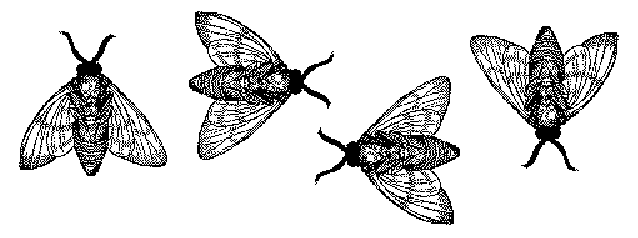
\includegraphics{flies}
%\caption{A sample black and white graphic (.pdf format)
%that needs to span two columns of text.}
%\label{fig:flies}
%\end{figure*}
%
%
%Note that only {\textbf{.pdf}} files were used; if you want to include
%{\textbf{.ps}} or {\textbf{.eps}} formats, you can use the
%\texttt{{\char'134}epsfig} or \texttt{{\char'134}psfig}
%commands as appropriate for the different file types.
%
%\subsection{Theorem-like Constructs}
%Other common constructs that may occur in your article are
%the forms for logical constructs like theorems, axioms,
%corollaries and proofs.  There are
%two forms, one produced by the
%command \texttt{{\char'134}newtheorem} and the
%other by the command \texttt{{\char'134}newdef}; perhaps
%the clearest and easiest way to distinguish them is
%to compare the two in the output of this sample document:
%
%This uses the \textbf{theorem} environment, created by
%the\linebreak\texttt{{\char'134}newtheorem} command:
%\newtheorem{theorem}{Theorem}
%\begin{theorem}
%Let $f$ be continuous on $[a,b]$.  If $G$ is
%an antiderivative for $f$ on $[a,b]$, then
%\begin{displaymath}\int^b_af(t)dt = G(b) - G(a).\end{displaymath}
%\end{theorem}
%
%The other uses the \textbf{definition} environment, created
%by the \texttt{{\char'134}newdef} command:
%\newdef{definition}{Definition}
%\begin{definition}
%If $z$ is irrational, then by $e^z$ we mean the
%unique number which has
%logarithm $z$: \begin{displaymath}{\log e^z = z}\end{displaymath}
%\end{definition}
%
%Two lists of constructs that use one of these
%forms is given in the
%\textit{Author's  Guidelines}.
%
%
%There is one other similar construct environment, which is
%already set up
%for you; i.e. you must \textit{not} use
%a \texttt{{\char'134}newdef} command to
%create it: the \textbf{proof} environment.  Here
%is a example of its use:
%\begin{proof}
%Suppose on the contrary there exists a real number $L$ such that
%\begin{displaymath}
%\lim_{x\rightarrow\infty} \frac{f(x)}{g(x)} = L.
%\end{displaymath}
%Then
%\begin{align*}
%l&=\lim_{x\rightarrow c} f(x)
%= \lim_{x\rightarrow c}
%\left[ g{x} \cdot \frac{f(x)}{g(x)} \right ] \\
%&= \lim_{x\rightarrow c} g(x) \cdot \lim_{x\rightarrow c}
%\frac{f(x)}{g(x)} = 0\cdot L = 0,
%\end{align*}
%which contradicts our assumption that $l\neq 0$.
%\end{proof}
%
%Complete rules about using these environments and using the
%two different creation commands are in the
%\textit{Author's Guide}; please consult it for more
%detailed instructions.  If you need to use another construct,
%not listed therein, which you want to have the same
%formatting as the Theorem
%or the Definition\cite{salas:calculus} shown above,
%use the \texttt{{\char'134}newtheorem} or the
%\texttt{{\char'134}newdef} command,
%respectively, to create it.
%
%\subsection*{A {\secit Caveat} for the \TeX\ Expert}
%Because you have just been given permission to
%use the \texttt{{\char'134}newdef} command to create a
%new form, you might think you can
%use \TeX's \texttt{{\char'134}def} to create a
%new command: \textit{Please refrain from doing this!}
%Remember that your \LaTeX\ source code is primarily intended
%to create camera-ready copy, but may be converted
%to other forms -- e.g. HTML. If you inadvertently omit
%some or all of the \texttt{{\char'134}def}s recompilation will
%be, to say the least, problematic.

%\section{Conclusions}
%We demonstrated YCSB-D, a tool that %can simulate dynamic variations in YCSB workload. YCSB-D
% can be used to benchmark target systems against dynamic workload variation patterns, by simulating any possible parallel
% workload variation pattern, without manually starting the YCSB client on each node in the cluster.  We demonstrate that YCSB-D can be used to evaluate the adaptability of automated tuning systems with respect to a given SLA.  %The tool is integrated with OptCon, a tool that can predict the matching consistency level, which satisfied the latency and staleness thresholds given in the SLA. We use the YCSB tool to demonstrate OptCon's adaptability to varying workload.


%\end{document}  % This is where a 'short' article might terminate

% ensure same length columns on last page (might need two sub-sequent latex runs)
\balance

%ACKNOWLEDGMENTS are optional
%\section{Acknowledgments}
%This section is optional; it is a location for you
%to acknowledge grants, funding, editing assistance and
%what have you.  In the present case, for example, the
%authors would like to thank Gerald Murray of ACM for
%his help in codifying this \textit{Author's Guide}
%and the \textbf{.cls} and \textbf{.tex} files that it describes.


% The following two commands are all you need in the
% initial runs of your .tex file to
% produce the bibliography for the citations in your paper.
{\footnotesize
\bibliographystyle{abbrv}
\bibliography{Consistency}}  % vldb_sample.bib is the name of the Bibliography in this case
% You must have a proper ".bib" file
%  and remember to run:
% latex bibtex latex latex
% to resolve all references

%\subsection{References}
%Generated by bibtex from your ~.bib file.  Run latex,
%then bibtex, then latex twice (to resolve references).
%
%%APPENDIX is optional.
%% ****************** APPENDIX **************************************
%% Example of an appendix; typically would start on a new page
%%pagebreak
%
%\begin{appendix}
%You can use an appendix for optional proofs or details of your evaluation which are not absolutely necessary to the core understanding of your paper.
%
%\section{Final Thoughts on Good Layout}
%Please use readable font sizes in the figures and graphs. Avoid tempering with the correct border values, and the spacing (and format) of both text and captions of the PVLDB format (e.g. captions are bold).
%
%At the end, please check for an overall pleasant layout, e.g. by ensuring a readable and logical positioning of any floating figures and tables. Please also check for any line overflows, which are only allowed in extraordinary circumstances (such as wide formulas or URLs where a line wrap would be counterintuitive).
%
%Use the \texttt{balance} package together with a \texttt{\char'134 balance} command at the end of your document to ensure that the last page has balanced (i.e. same length) columns.
%
%\end{appendix}
%
%

\end{document}
